\documentclass[answers]{exam}
\input{global}
\input{problem-sets}
%...UNIT 1: CONSTANT VELOCITY

\newcommand{\xygraphI}[3]{
\begin{tikzpicture}
    \begin{axis}[height=7.7cm,width=8.5cm,
        axis lines=center,
        ylabel={$y$},
        xlabel={$x$},
        ymin=-10,ymax=10,
        xmin=-10,xmax=10,
        ytick={-10,-8,...,10},
        xtick={-10,-8,...,10},
        grid=both, 
        minor y tick num=1,
        minor x tick num=1,
    ]
        \addplot[thick,domain=-10:10] {#1*x + #2};
        \ifprintanswers
            \addplot[red,only marks,mark=*] coordinates{#3};
        \fi
    \end{axis}
\end{tikzpicture}
}


\newcommand{\distancegraphI}[1]{
    \begin{tikzpicture}
        \begin{axis}[height=6.5cm,width=6.8cm,
            axis lines=left,
            xlabel = {Time (hours)},
            ylabel = {Distance (miles)},
            ymin=0, ymax=100,
            xmin=0, xmax=5,
            ytick={0,10,...,100},
            xtick={0,1,...,5},
            minor x tick num=1,
            grid=both,
            ]
            \addplot[very thick,domain=0:5] {#1*x};
        \end{axis}
    \end{tikzpicture}
}

\newcommand{\positiongraphI}[3]{
    \begin{tikzpicture}
        \begin{axis}[height=5.6cm,width=6.5cm,
            axis lines=left,
            xlabel = {Time (s)},
            ylabel = {Position (m)},
            ymin=0, ymax=20,
            xmin=0, xmax=14,
            ytick={0,4,...,20},
            xtick={0,2,...,14},
            minor y tick num=3,
            minor x tick num=1,
            grid=both,
            ]
            \addplot[very thick,domain=0:14] {#1*x + #2};
            \ifprintanswers
                \addplot[red,only marks,mark=*] coordinates{#3};
            \fi
        \end{axis}
    \end{tikzpicture}

%...AI-CHATBOT PROMPT:
% In an xy plane, the y limits are 0 to 20, and the x limits are 0 to 14. Give me 5 excellent linear equations (y = mx + b) for students to practice slope calculations. Output the results in the form \positiongraphI{m}{b}{coordinates} where coordinates should be in the form (x1,y1)(x2,y2), representing 2 points on the line for calculating slope. 
}

\newcommand{\positionfigureI}[1]{
\begin{center}
    \begin{tikzpicture}[y=1cm,x=1cm]
        \foreach \x in {-5,-4,...,5} {
            \draw[ultra thin] (\x,-1mm) -- (\x,1mm) node[below=2mm] {$\x$};
        }
        \draw[->] (-5,0) -- (5,0) node[below=6mm,pos=0.5] {Position (m)};
        \node[above] at (#1,0) {\Strichmaxerl[2]};
        \ifprintanswers
            \draw[very thick,->,red] (0,0.7) -- ++(#1,0) node[above,pos=0.5] {$\vec{x}$};
        \fi
    \end{tikzpicture}  
\end{center}
}

\newcommand{\positionfigureII}[2]{
\begin{center}
\begin{tikzpicture}[y=1cm,x=1cm]
    \foreach \x in {-5,-4,...,5} {
        \draw[ultra thin] (\x,-1mm) -- (\x,1mm) node[below=3mm] {$\x$};
    }
    \draw[->] (-5,0) -- (5,0) node[below=7mm,pos=0.5] {Position (m)};
    \fill (#1,0) circle (1mm) node[above=1mm] {A};
    \fill (#2,0) circle (1mm) node[above=1mm] {B};
\end{tikzpicture}
\end{center}
}


\newcommand{\positionfigureIII}[4]{
\begin{center}
\begin{tikzpicture}[y=3mm,x=8mm]
    \draw[black!10,xstep=1,ystep=2] (0,0) grid (12,4);
    \foreach \x in {0,1,...,12} {
        \draw[ultra thin] (\x,-1mm) -- (\x,1mm) node[below=3mm] {$\x$};
    }
    \draw[->] (0,0) -- (12,0) node[right=1mm] {$x$ (m)};
    \draw[ultra thick,->,rounded corners=0.7mm] (#1,1)
        -- (#2,1) 
        -- (#2,2) 
        -- (#3,2) 
        -- (#3,3) 
        -- (#4,3);
    \node[fill=black!10] at (#1,-3) {$x_i$};
    \node[above=1mm,fill=black!10] at (#4,4) {$x_f$};
\end{tikzpicture}
\end{center}
}

\newcommand{\positionfigureIV}[2]{
    \begin{center}
    \begin{tikzpicture}[y=1.4mm,x=1.4mm]
        \foreach \x in {-50,-40,...,50} {
            \draw[ultra thin] (\x,-1mm) -- (\x,1mm) node[below=3mm] {$\x$};
        }
        \foreach \x in {-45,-35,...,45} {
            \draw[ultra thin] (\x,-0.8mm) -- (\x,0.8mm);
        }
        \draw[->] (-50,0) -- (50,0) node[below=7mm,pos=0.5] {Position (m)};
        \fill (#1,0) circle (1mm) node[above=1mm] {A};
        \fill (#2,0) circle (1mm) node[above=1mm] {B};
    \end{tikzpicture}
    \end{center}
}

\newcommand{\positionfigureV}[6]{
    %...PRO TIP: Type the following into ChatGPT:
    % Generate 5 integers between -10 to 10 (inclusive) such that the absolute value of the sum of the 5 integers is less than or equal to 10. Print each of the integers in each of the first 5 curly brackets below. Calculate the maximum displacement from equilibrium and, if it's greater than 10, enter it in the 6th curly bracket; otherwise enter 10 for the 6th curly bracket. Do not output in markdown; I just want the verbatim text: \positionfigureV{}{}{}{}{}{}
    
    \begin{tikzpicture}[x=4mm,y=4mm]
        \draw[step=1,lightgray] (-10,0) grid (10,4);
        \draw[->,line width=0.6mm,-{Triangle}] (0,4) -- ++(#5,0);
        \draw[->,line width=0.6mm,-{Triangle}] (0,3) -- ++(#4,0);
        \draw[->,line width=0.6mm,-{Triangle}] (0,2) -- ++(#3,0);
        \draw[->,line width=0.6mm,-{Triangle}] (0,1) -- ++(#2,0);
        \draw[->,line width=0.6mm,-{Triangle}] (0,0) -- ++(#1,0);
        \node[below] at (current bounding box.south) {Figure 1: Displacement vectors.};
    \end{tikzpicture}
    
    \smallskip
    
    \begin{tikzpicture}[x=4mm,y=4mm]
        \draw[step=1,lightgray] (-#6,0) grid (#6,4);
        \draw (0,0) node {\scriptsize $|$} node[below=2pt] {$0$};
            \begin{scope}[red,opacity={\ifprintanswers 1\else 0\fi}]
                \draw[->,line width=0.3mm,-{Triangle}] ({#1+#2+#3+#4},4) -- ++(#5,0);
                \draw[->,line width=0.3mm,-{Triangle}] ({#1+#2+#3},3) -- ++(#4,0);
                \draw[->,line width=0.3mm,-{Triangle}] ({#1+#2},2) -- ++(#3,0);
                \draw[->,line width=0.3mm,-{Triangle}] (#1,1) -- ++(#2,0);
                \draw[->,line width=0.3mm,-{Triangle}] (0,0) -- ++(#1,0);
                \pgfmathsetmacro{\vecsum}{#1+#2+#3+#4+#5}
        
                \pgfmathtruncatemacro{\iszero}{(\vecsum==0)}
                
                \ifnum\iszero=1
                    \node[above] at (0,4.6) {vector sum is zero};
                \else
                    \draw[->,line width=0.6mm,-{Triangle}] (0,4.8) -- ++(\vecsum,0)
                        node[above=1mm,pos=0.5] {vector sum};
                \fi
        \end{scope}
        \node[below] at (current bounding box.south) {Figure 2: Head-to-tail addition and vector sum.};
    \end{tikzpicture}
}

\newcommand{\positionfigureVI}[1]{
\begin{tikzpicture}[y=6mm,x=6mm]
    \draw[black!20,step=1] (0,0) grid (24,2);  
    \draw[|-|] (0,-0.3) -- ++(1,0) node[below] {\small 1 meter};
    \ifprintanswers
    \foreach \x in {0,#1,...,24}{
        \fill[red] (\x,1) circle (0.9mm);
    }
    \fi
\end{tikzpicture}
}

\newcommand{\positiongraphIII}[6]{
    %...Generates a quadrant I position vs. time with linear function.
    % #1 = velocity (slope)
    % #2 = initial position (y-intercept)
\begin{tikzpicture}
\begin{axis}[height=5.9cm,width=6.4cm,
    axis lines=left,
    xlabel = {Time (s)},
    ylabel = {Position (m/s)},
    ymin=0, ymax=10,
    xmin=0, xmax=10,
    ytick={0,1,...,10},
    xtick={0,1,...,10},
    grid = both,
    clip=true,
    legend style={at={(1.1,0.85)}}
    % set layers
    ]
    \addplot[very thick,black,domain=0:10] {#1*\x + #2};
    \addlegendentry{A} % <-- Legend for the first plot
    
    \addplot[densely dashed,very thick,black,domain=0:10] {#3*\x + #4};
    \addlegendentry{B} 

    \addplot[only marks, mark=*,mark size=1.5pt,black,domain=0:10] {#5*\x + #6};
    \addlegendentry{C} 
    \end{axis}
\end{tikzpicture}
}

\newcommand{\velocitygraph}[2]{
    \begin{tikzpicture}
        \begin{axis}[height=6cm,width=7cm,
            axis y line=left,
            axis x line=center,
            xlabel = {Time (s)},
            ylabel = {Velocity (m/s)},
            ymin=-5, ymax=5,
            xmin=0, xmax=10,
            ytick={-5,-4,...,5},
            xtick={0,2,...,10},
            grid=both,
            minor x tick num = 1,
            x label style={at={(axis description cs:1,0.5)},right=1mm},
            clip=false
        ]
            \addplot[very thick,black,domain=0:#2] {#1};
            \ifprintanswers
                \begin{pgfonlayer}{background}
                    \fill[red!12] (0,0) rectangle (#2,#1);
                \end{pgfonlayer}
            \fi
            \end{axis}
    \end{tikzpicture}
}

%...AI-CHATBOT PROMPT:
%Generate a random integer between -5 to 5 (inclusive), and another one between 5 and 10 (inclusive). Output the results in the form \velocitygraph{a}{b} where a and b are the generated numbers.




%..UNIT 2: ACCELERATION

\newcommand{\velocitytableI}[4]{%
    % #1 = initial velocity
    % #2 = acceleration
    % #3 = initial time
    % #4 = change in time
\begin{tabular}{|c|c|}
    \hline
    \thead{\bfseries Velocity (m/s)} & \thead{\bfseries Time (s)} \\ \hline
    $\fpeval{#1 + #2*(#3 + 0*#4)}$ & \fpeval{#3 + 0*#4} \\ \hline
    $\fpeval{#1 + #2*(#3 + 1*#4)}$ & \fpeval{#3 + 1*#4} \\ \hline
    $\fpeval{#1 + #2*(#3 + 2*#4)}$ & \fpeval{#3 + 2*#4} \\ \hline
    $\fpeval{#1 + #2*(#3 + 3*#4)}$ & \fpeval{#3 + 3*#4} \\ \hline
    $\fpeval{#1 + #2*(#3 + 4*#4)}$ & \fpeval{#3 + 4*#4} \\ \hline
\end{tabular}
}



\newcommand{\positiontableI}[5]{%
    % #1 = initial position
    % #2 = initial velocity
    % #3 = initial time
    % #4 = change in time
    % #5 = acceleration
\begin{tabular}{|c|c|}
    \hline
    \thead{\bfseries Position (m)} & \thead{\bfseries Time (s)} \\ \hline
    $\fpeval{#1 + #2*(#3 + 0*#4) + 0.5*#5*(#3 + 0*#4)^2}$ & \fpeval{#3 + 0*#4} \\ \hline
    $\fpeval{#1 + #2*(#3 + 1*#4) + 0.5*#5*(#3 + 1*#4)^2}$ & \fpeval{#3 + 1*#4} \\ \hline
    $\fpeval{#1 + #2*(#3 + 2*#4) + 0.5*#5*(#3 + 2*#4)^2}$ & \fpeval{#3 + 2*#4} \\ \hline
    $\fpeval{#1 + #2*(#3 + 3*#4) + 0.5*#5*(#3 + 3*#4)^2}$ & \fpeval{#3 + 3*#4} \\ \hline
    $\fpeval{#1 + #2*(#3 + 4*#4) + 0.5*#5*(#3 + 4*#4)^2}$ & \fpeval{#3 + 4*#4} \\ \hline
\end{tabular}
}

\NewDocumentCommand{\velocitygraphI}{m m o}{
    % Produces a line on a velocity vs time graph.
    % #1 = slope (acceleration) 
    % #2 = y-intercept (initial velocity)
    % #3 [optional] = sample coordinates (x1,y1)(x2,y2) for finding slope
\begin{tikzpicture}
\begin{axis}[height=6cm,width=6.4cm,
    axis y line=left,
    axis x line=center,
    ylabel = {Velocity (m/s)},
    xlabel = {Time (s)},
    ymin=-8, ymax=8,
    xmin=0, xmax=10,
    ytick={-8,-6,...,8},
    xtick={0,1,...,10},
    grid = both,
    minor y tick num=1,
    ]
    \addplot[very thick,black,domain=0:10] {#1*\x + #2};
    \ifprintanswers
            % \IfValueT checks if the 3rd argument was actually provided
            \IfValueT{#3}{
                \addplot[red,only marks,mark=*] coordinates{#3};
            }
        \fi
    \end{axis}
\end{tikzpicture}

%...AI CHATBOT PROMPT:
% A velocity vs. time graph has y limits -8 to 8 and x limits 0 to 10. Generate a linear function for students to practice calculating acceleration. Output the result in the form \velocitygraphI{m}{b}{(x1,y1)(x2,y2)} where m is the slope (acceleration), b is the y-intercept (initial velocity), and (x1,y1)(x2,y2) are two coordinates on the line used to calculate slope. Negative accelerations are acceptable.
}

\newcommand{\positiongraphII}[3]{
    % Generates a position vs. time graph for uniform acceleration motion.
    %...Inspired by https://ophysics.com/k4.html
    % #1 = initial position
    % #2 = initial velocity
    % #3 = acceleration
\begin{tikzpicture}
    \begin{axis}[height=6cm,width=5cm,
        axis y line=left,
        axis x line=center,
        ylabel={Position (m)},
        xlabel={Time (s)},
        ymin=-4,ymax=4,
        xmin=0,xmax=4,
        ytick={-4,-3,...,4},
        xtick={0,1,...,4},
        grid=both,
        x label style={at={(axis description cs: 1,0.5)},right=1mm},
    ]
        \addplot[very thick,domain=0:4] {#1 + #2*x + 0.5*#3*x^2};        
    \end{axis}
\end{tikzpicture}    
}

\newcommand{\velocitygraphII}[2]{
    %...Generates a minimalistic v vs. t graph.
    % #1 = initial velocity (y-intercept)
    % #2 = acceleration (slope)
    %... See https://ophysics.com/k4.html
\begin{tikzpicture}[y=5mm,x=7mm]
    \draw[->] (0,-4.4) -- (0,4.4) node[left,pos=0.9] {$v$} node[pos=0.5,left] {\footnotesize $0$};
    \draw[->] (0,0) -- (4.4,0) node[right] {$t$};
    \draw[very thick,domain=0:4] plot(\x,{#1 + #2*\x});
\end{tikzpicture}
}


\newcommand{\velocitygraphIII}[3]{
    %...Generates a quadrant I velocity vs. time with linear function.
    % #1 = acceleration (slope)
    % #2 = initial velocity (y-intercept)
    % #3 = final time (where line stops)
\begin{tikzpicture}
\begin{axis}[height=6cm,width=6.4cm,
    axis lines=left,
    xlabel = {Time (s)},
    ylabel = {Velocity (m/s)},
    ymin=0, ymax=10,
    xmin=0, xmax=10,
    ytick={0,1,...,10},
    xtick={0,1,...,10},
    grid = both,
    clip=true,
    % set layers
    ]
    \addplot[very thick,black,domain=0:#3] {#1*\x + #2};
    \ifprintanswers
    \begin{pgfonlayer}{background}
        \fill[red!10] (0,#2) -- (#3,{#1*#3+#2}) -- (#3,0) -- (0,0) -- cycle;
    \end{pgfonlayer}
    \fi
    \end{axis}
\end{tikzpicture}

%...AI CHATBOT PROMPT:
% A velocity vs. time graph has y limits 0 to 10 and x limits 0 to 10. Generate a linear function for students to practice calculating displacement (as area under the curve). Output the result in the form \velocitygraphIII{m}{b} where m is the slope (acceleration) and b is the y-intercept (initial velocity). Negative accelerations are acceptable.
}

\newcommand{\triangleI}[3]{%
    % #1 = base
    % #2 = height
    % #3 = a parameter to control figure size
    \begin{tikzpicture}[y=1mm*#3,x=1mm*#3]
        \draw[thick,fill=black!10] (-0.5*#1,0) -- (0.5*#1,0) -- (0,#2) -- cycle;
        \draw[densely dashed] (0,0) -- (0,#2) node[pos=0.4,right] {#2};
        \draw[|-|] (-0.5*#1,-2mm) -- (0.5*#1,-2mm) node[below,pos=0.5] {#1};
    \end{tikzpicture}
}

\newcommand{\triangleII}[3]{%
    % #1 = base
    % #2 = height
    % #3 = a parameter to control figure size
    \begin{tikzpicture}[y=1mm*#3,x=1mm*#3]
        \draw[thick,fill=black!10] (0,0) -- (#1,0) node[below,pos=0.5] {#1} -- (#1,#2) node[right,pos=0.5] {#2} -- cycle;
    \end{tikzpicture}
}

\firstpageheader{{Name:\enspace\makebox[6cm]{\hrulefill}}\\Physics}{}
{Problems\\Unit 2: Changing Motion}
\runningheader{Physics}{}{Problems on Unit 2: Changing Motion}

\setlength{\columnseprule}{0pt}

\usepackage{adjustbox}
\usepackage{xfp}

%...Speedometer
\newcommand{\speedometer}[3]{%
    % #1: X-shift (y is fixed at 2) (e.g., 1)
    % #2: Needle rotation angle (e.g., 20)
    % #3: Top label (e.g., \texttt{Speed})
    % #4: Bottom readout (e.g., \textsf{32.0\,m/s})
    \begin{scope}[shift={#1},x=1cm,y=1cm,scale=0.8,transform shape,overlay]
        \draw (0,0) circle (1);
        \foreach \x in {340,360,...,560} {
            \coordinate (P) at ({cos(\x)},{sin(\x)});
            \draw[ultra thick,gray] (P) -- ($(P)!0.16!(0,0)$);
        }
        \foreach \x in {350,370,...,550} {
            \coordinate (P) at ({cos(\x)},{sin(\x)});
            \draw[thick,gray] (P) -- ($(P)!0.08!(0,0)$);
        }
        \fill (0,0) circle (0.02);
        \draw[fill=lightgray,rotate={#2},red!60] (0,0.02) rectangle (0.975,-0.02);
        \node at (0,0.4) {\texttt{Speed}};
        \draw[rounded corners] (-0.65,-0.75) rectangle ++(1.3,0.5) node[pos=0.5] {\textsf{#3\,m/s}};
    \end{scope}
}

% \usepackage[explicit]{titlesec}
% \renewcommand{\thesubsection}{\arabic{subsection}}
% \titleformat{\subsection}
%   {\normalfont\large\bfseries} % The font styling (bold, large)
%   {}                           % Leave the standard label empty
%   {0pt}                        % Spacing between label and title
%   {#1 \thesubsection}


\begin{document}

\subsection*{Lab: Galileo's Ramp Experiment}

\noindent \textit{Materials:} 
\vspace{1ex}

track, steel ball, metronome, tape strips, meterstick

\begin{center}
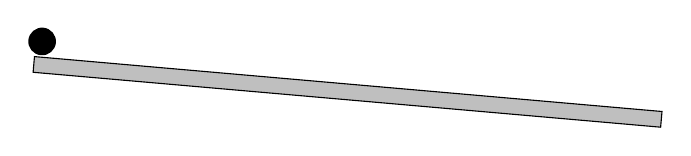
\begin{tikzpicture}[x=8cm]
    \begin{scope}[rotate=-5]
        \draw[fill=lightgray] (0,-0.1) rectangle (1,0.1);
        \fill (0.01,0.3) circle (5pt);
    \end{scope}
\end{tikzpicture}
\end{center}

\noindent \textit{Procedure:}

\begin{enumerate}[itemsep=0pt,topsep=2pt]
\item Incline the track so that the origin (\SI{0}{cm}) is at a greater vertical position than the track's end (\SI{120}{cm}).
\item The teacher sets a metronome at 60\,BPM, yielding 1 beat per second.
\item Release the ball from rest at 0\,cm, exactly on the sound of a beat. Call this ``Beat 0.''
\item For each subsequent beat, place a tape strip on the track, at the ball’s location for that beat. Once the ball's positions are all marked, \textbf{call your teacher} to inspect your tape strips.
\item After teacher approval, sketch a prediction of what the the ball's position $x$ and velocity $v$ could look like as a functions of time $t$, based on the distribution of tape across the track.

\begin{center}
\begin{tikzpicture}[x=3cm,y=3cm]
    \draw[->] (0,0) -- (0,1.2) node[left,pos=0.9] {\large $x$};
    \draw[->] (0,0) -- (1.2,0) node[right] {\large $t$};
    \ifprintanswers
        \draw[ultra thick,smooth,domain=0:1,red] plot(\x,\x*\x);
    \fi
\end{tikzpicture}
\hspace{1cm}
\begin{tikzpicture}[x=3cm,y=3cm]
    \draw[->] (0,0) -- (0,1.2) node[left,pos=0.9] {\large $v$};
    \draw[->] (0,0) -- (1.2,0) node[right] {\large $t$};
    \ifprintanswers
        \draw[ultra thick,smooth,domain=0:1,red] plot(\x,\x);
    \fi
\end{tikzpicture}
\end{center}

\item Record tape positions in the table below. Then, graph your data. (Remember, each metronome beat represents 1 second of time.)

\begin{center}
\begin{minipage}{4cm}
\centering
\def\arraystretch{1.8}
\begin{tabular}{|w{c}{1.5cm}|w{c}{1.5cm}|}
    \hline
    \thead{\bfseries Time\\ \bfseries (s)} & \thead{\bfseries Position\\ \bfseries (cm)} \\ \hline
    0 & 0 \\ \hline 
    1 & \ans{5} \\ \hline 
    2 & \ans{19} \\ \hline 
    3 & \ans{41} \\ \hline 
    4 & \ans{72} \\ \hline 
    5 & \ans{118} \\ \hline 
\end{tabular}
\vspace{5mm}
\end{minipage}%
\hspace{5mm}
\begin{minipage}{10.5cm}
\centering
\begin{tikzpicture}
    \begin{axis}[height=8cm,width=9cm,
        ylabel={Position (cm)},
        xlabel={Time (s)},
        ymin=0,ymax=120,
        xmin=0,xmax=5,
        ytick={0,20,...,120},
        xtick={0,1,...,5},
        axis lines=left,
        grid=both,
        minor y tick num=1,
        minor x tick num=1,
        clip=false
    ]
    \ifprintanswers
    \addplot[mark=*,only marks,red] coordinates{(0,0)(1,5)(2,19)(3,41)(4,72)(5,118)};
    \fi
    \end{axis}
\end{tikzpicture}
\end{minipage}
\end{center}

\clearpage

\item Use a meterstick to measure displacements $\left(\Delta x\right)$ between adjacent tape strips, from left to right. Record your data below. In column 3, calculate the ratio of subsequent displacements to the first one.
\end{enumerate}



\vspace{-1.5em}

\begin{EnvUplevel}
\def\arraystretch{1.8}
\begin{center}
\begin{tabular}{|w{c}{3cm}|w{l}{5cm}|w{l}{4cm}|}
    \hline
    \thead{\bfseries Time Interval} & \thead{\bfseries Interval Displacement (cm)} & \thead{\bfseries Ratio $\Delta x_n/\Delta x_1$} \\ \hline
    Beat 0 to 1 & $\Delta x_1 =$ \ans{5} & $\Delta x_1 \div \Delta x_1 = 1.0$ \\[1ex] \hline 
    Beat 1 to 2 & $\Delta x_2 =$ \ans{14} & $\Delta x_2 \div \Delta x_1 = \ans{2.8}$ \\[1ex] \hline 
    Beat 2 to 3 & $\Delta x_3 =$ \ans{22} & $\Delta x_3 \div \Delta x_1 = \ans{4.4}$ \\[1ex] \hline 
    Beat 3 to 4 & $\Delta x_4 =$ \ans{31} & $\Delta x_4 \div \Delta x_1 = \ans{6.2}$ \\[1ex] \hline 
    Beat 4 to 5 & $\Delta x_5 =$ \ans{46} & $\Delta x_5 \div \Delta x_1 = \ans{9.2}$ \\[1ex] \hline 
\end{tabular}
\end{center}
\end{EnvUplevel}

\noindent \textit{Analysis:}

\begin{questions}
\question
In \textit{Procedure} step 6, is the position changing at a constant rate? What does this indicate about velocity?

\ifprintanswers
\textcolor{red}{No. While position is increasing, the gaps between each position are increasing with time. This means velocity is increasing with time.}
\else
\fillwithlines{21mm}
\fi

\question 
Acceleration is the rate at which velocity changes with time. Is the steel ball accelerating? How do you know?

\ifprintanswers
\textcolor{red}{We know the velocity is changing with time because we observed it go from rest to moving at a faster speed towards the end of the track.}
\else
\fillwithlines{21mm}
\fi


\question 
Describe the shape of the position-vs-time graph. Is it linear, like with the Dune Buggy from Unit 1?

\ifprintanswers
\textcolor{red}{The shape of the graph is curved, like a parabola. It's not linear like the Dune Buggy lab, but quadratic.}
\else
\fillwithlines{21mm}
\fi

\question
Notice the patterns in \textit{Procedure} step 7. Use those trends to complete the sentences below. 

\begin{itemize}[itemsep=2pt]
    \item The interval displacements \fillin[are increasing][8cm]\ as the beats of time increase from 0 to 5.
    \item The ratios of displacements $\left(\Delta x_n/\Delta x_1\right)$ \fillin[are also increasing][7cm] with time.
    \item These observations indicate that velocity \fillin[is increasing with time][8cm].
\end{itemize}

\question
\begin{parts}
\part In what ways are the motion of the Steel Ball different than the motion of the Dune Buggy?

\ifprintanswers
\textcolor{red}{The Steel Ball started from rest and increased in velocity throughout the track. The Dune Buggy started with and maintained constant velocity throughout its motion. Also, the ball's position-vs-time graph is curved (quadratic), whereas the Dune Buggy's graph is linear.}
\else
\fillwithlines{14mm}
\fi

\part In what ways are the motions similar?


\ifprintanswers
\textcolor{red}{Both objects changed position over time, as they moved across the track. Both objects moved in the positive direction. Both objects were subject to measurements of time.}
\else
\fillwithlines{14mm}
\fi
\end{parts}
\end{questions}


\clearpage

\noindent {\bfseries Part II: Ramp Experiment with Vernier}. 

\begin{itemize}[topsep=2pt,itemsep=0pt]
    \item Step 1: Go to \href{https://graphicalanalysis.app/}{\texttt{graphicalanalysis.app}}. Click \textsf{Sensor Data Collection} and connect cart with \textsf{WIRELESS}. 
    \item Step 2: Click 
        \tikz{\draw[thick] (0,0) rectangle (2.4mm,2.4mm); 
            \draw[thick] (1.2mm,2.4mm) -- ++(0,-2.4mm);
            \draw[thick] (1.2mm,1.2mm) -- ++(1.2mm,0);
            }
        and set \textsf{Number of Graphs} to \textsf{3 graphs}.
    \item Step 3: Click \tikz{\node at (0,0) {\large \bfseries \ldots};}, click \textsf{App Preferences}, and click 
    \tikz[x=1mm,y=1mm]{\fill (0,0) circle (1);
        \begin{scope}[x=1.15mm,y=1.15mm]
            \foreach \x in {0,45,...,315}{
            \draw[thick,rotate around={\x:({cos(\x)},{sin(\x)})}] ({cos(\x)},{sin(\x)}) -- ++(0.4,0);}
        \end{scope}
        ;} (toggle light mode).
\end{itemize}

\vspace{2pt}

\begin{questions}
\question
Click \textsf{COLLECT}. Release the cart from rest at 0\,cm.


\begin{center}
\begin{tikzpicture}[y=0.6mm,x=0.8mm,rotate=-8,transform shape]
    \draw[fill=black!8] (0,-1mm) rectangle (120,1mm);
    \foreach \x in {0,10,...,120} {
        \draw[ultra thin] (\x,-1mm) -- (\x,1mm) node[below=2mm] {\scriptsize $\x$};
    }
    \foreach \x in {0,2,...,120} {
        \draw[ultra thin] (\x,-0.5mm) -- (\x,0.5mm);
    }
    \draw[->] (0,0) -- (120,0) node[below=4mm,pos=0.5] {\small Position (cm)};
    \node at (5,4.2mm) {\resizebox{1cm}{!}{\reflectbox{\usym{1F699}}}};
    \draw[line width=1mm,-{Triangle[scale=0.7]}] (14,10) -- ++(10,0) node[below,pos=0.3] {\textsf{x}\footnotesize +};
\end{tikzpicture} 
\end{center}


\begin{parts}
\part Is the cart speeding up or slowing down? \fillin[speeding up][6cm]

\part Draw a motion map for the cart. 
\tikz[x=7mm,y=7mm]{
    \draw (-1.6,-0.3) rectangle (12,0.3);
    \node at (-1,0) {\SI{0}{cm}};
    \node at (11.2,0) {\SI{120}{cm}};
    \ifprintanswers
    \draw[red,domain=0:10,mark=*,only marks, samples=10,mark size=2pt] plot({0.1*\x^2},0);
    \else
    \draw[white,domain=0:10,mark=*,only marks, samples=10,mark size=2pt] plot({0.1*\x^2},0);
    \fi
}


\part Sketch the position vs.\,time, the velocity vs.\,time, and acceleration vs.\,time graphs.

\begin{center}
\begin{tikzpicture}[x=2.5cm,y=2.5cm]
        \draw (0,-0.6) -- (0,0.6) node[rotate=90,pos=0.5,above] {Position (m)};
        \draw (0,0) -- (1.2,0);
        \node[below] at (0.6,-0.6) {Time (s)};
    % \ifprintanswers
    %     \draw[very thick,red,domain=0:1,smooth] plot(\x,\x^2);
    % \fi
    \begin{scope}[shift={(2,0)}]
        \draw (0,-0.6) -- (0,0.6) node[rotate=90,pos=0.5,above] {Velocity (m/s)};
        \draw (0,0) -- (1.2,0);
        \node[below] at (0.6,-0.6) {Time (s)};
        \ifprintanswers
            \draw[very thick,red,domain=0:1,smooth] plot(\x,0.5*\x);
        \fi
    \end{scope}
    \begin{scope}[shift={(4,0)}]
        \draw (0,-0.6) -- (0,0.6) node[rotate=90,pos=0.5,above] {Acceleration (\SI{}{m/s^2})};
        \draw (0,0) -- (1.2,0);
        \node[below] at (0.6,-0.6) {Time (s)};
        \ifprintanswers
            \draw[very thick,red,domain=0:1,smooth] plot(\x,0.25);
        \fi
    \end{scope}
\end{tikzpicture}
\end{center}

\part Is the velocity positive or negative? How do you know? 

\begin{solution}
    Positive. The object moves away from the origin.
\end{solution}

\ifprintanswers
\else
\fillwithlines{7mm}
\fi


% \fillin[positive; motion is away from the origin][6cm]
\end{parts}

\question
Click \textsf{COLLECT}. Give the cart an initial push up the ramp and stop it at its highest point.


\begin{center}
\begin{tikzpicture}[y=0.6mm,x=0.8mm,rotate=8,transform shape]
    \draw[fill=black!8] (0,-1mm) rectangle (120,1mm);
    \foreach \x in {0,10,...,120} {
        \draw[ultra thin] (\x,-1mm) -- (\x,1mm) node[below=2mm] {\scriptsize $\x$};
    }
    \foreach \x in {0,2,...,120} {
        \draw[ultra thin] (\x,-0.5mm) -- (\x,0.5mm);
    }
    \draw[->] (0,0) -- (120,0) node[below=4mm,pos=0.5] {\small Position (cm)};
    \node at (5,4.2mm) {\resizebox{1cm}{!}{\reflectbox{\usym{1F699}}}};
    \draw[line width=1mm,-{Triangle[scale=0.7]}] (14,10) -- ++(10,0) node[below,pos=0.3] {\textsf{x}\footnotesize +};
\end{tikzpicture} 
\end{center}


\begin{parts}
\part Is the cart speeding up or slowing down? \fillin[slowing down][6cm]

\part Draw a motion map for the cart.
\tikz[x=7mm,y=7mm]{
    \draw (2,-0.3) rectangle (-11.8,0.3);
    \node at (1.1,0) {120\,cm};
    \node at (-11,0) {0\,cm};
    \ifprintanswers
    \draw[red,domain=0:10,mark=*,only marks, samples=10,mark size=2pt] plot({-0.1*\x^2},0);
    \else
    \draw[white,domain=0:10,mark=*,only marks, samples=10,mark size=2pt] plot({-0.1*\x^2},0);
    \fi
}

\part Draw the position vs.\,time, the velocity vs.\,time, and acceleration vs.\,time graphs.

\begin{center}
\begin{tikzpicture}[x=2.5cm,y=2.5cm]
        \draw (0,-0.6) -- (0,0.6) node[rotate=90,pos=0.5,above] {Position (m)};
        \draw (0,0) -- (1.2,0);
        \node[below] at (0.6,-0.6) {Time (s)};
    % \ifprintanswers
    %     \draw[very thick,red,domain=0:1,smooth] plot(\x,{-(\x-1)^2+1});
    % \fi
\begin{scope}[shift={(2,0)}]
    \draw (0,-0.6) -- (0,0.6) node[rotate=90,pos=0.5,above] {Velocity (m/s)};
    \draw (0,0) -- (1.2,0);
    \node[below] at (0.6,-0.6) {Time (s)};
    \ifprintanswers
        \draw[very thick,red,domain=0:1,smooth] plot(\x,-0.5*\x+0.5);
    \fi
\end{scope}
\begin{scope}[shift={(4,0)}]
    \draw (0,-0.6) -- (0,0.6) node[rotate=90,pos=0.5,above] {Acceleration (\SI{}{m/s^2})};
    \draw (0,0) -- (1.2,0);
    \node[below] at (0.6,-0.6) {Time (s)};
    \ifprintanswers
        \draw[very thick,red,domain=0:1,smooth] plot(\x,-0.25);
    \fi
\end{scope}
\end{tikzpicture}
\end{center}

\part Is the velocity positive or negative? How do you know? 

\begin{solution}
    Positive. The object moves away from the origin.
\end{solution}

\ifprintanswers
\else
\fillwithlines{7mm}
\clearpage
\fi

\end{parts}


\question
Click \textsf{COLLECT}. Roll the cart from 0\,cm to 120\,cm. Then, release it from rest at 120\,cm. 

\begin{center}
\begin{tikzpicture}[y=0.6mm,x=0.8mm,rotate=8,transform shape]
    \draw[fill=black!8] (0,-1mm) rectangle (120,1mm);
    \foreach \x in {0,10,...,120} {
        \draw[ultra thin] (\x,-1mm) -- (\x,1mm) node[below=2mm] {\scriptsize $\x$};
    }
    \foreach \x in {0,2,...,120} {
        \draw[ultra thin] (\x,-0.5mm) -- (\x,0.5mm);
    }
    \draw[->] (0,0) -- (120,0) node[below=4mm,pos=0.5] {\small Position (cm)};
    \node at (115,4.2mm) {\resizebox{1cm}{!}{\reflectbox{\usym{1F699}}}};
    \draw[line width=1mm,-{Triangle[scale=0.7]}] (95,10) -- ++(10,0) node[below,pos=0.3] {\textsf{x}\footnotesize +};
\end{tikzpicture} 
\end{center}


\begin{parts}
\part Is the cart speeding up or slowing down? \fillin[speeding up][6cm]

\part Draw a motion map for the cart.
\tikz[x=7mm,y=7mm]{
    \draw (2,-0.3) rectangle (-11.8,0.3);
    \node at (1.1,0) {120\,cm};
    \node at (-11,0) {0\,cm};
    \ifprintanswers
    \draw[red,domain=0:10,mark=*,only marks, samples=10,mark size=2pt] plot({-0.1*\x^2},0);
    \else
    \draw[white,domain=0:10,mark=*,only marks, samples=10,mark size=2pt] plot({-0.1*\x^2},0);
    \fi
}

\part Draw the position vs.\,time, the velocity vs.\,time, and acceleration vs.\,time graphs.

\begin{center}
\begin{tikzpicture}[x=2.5cm,y=2.5cm]
        \draw (0,-0.6) -- (0,0.6) node[rotate=90,pos=0.5,above] {Position (m)};
        \draw (0,0) -- (1.2,0);
        \node[below] at (0.6,-0.6) {Time (s)};
    % \ifprintanswers
    %     \draw[very thick,red,domain=0:1,smooth] plot(\x,{-\x^2+1});
    % \fi
\begin{scope}[shift={(2,0)}]
    \draw (0,-0.6) -- (0,0.6) node[rotate=90,pos=0.5,above] {Velocity (m/s)};
    \draw (0,0) -- (1.2,0);
    \node[below] at (0.6,-0.6) {Time (s)};
    \ifprintanswers
        \draw[very thick,red,domain=0:1,smooth] plot(\x,-0.5*\x);
    \fi
\end{scope}
\begin{scope}[shift={(4,0)}]
    \draw (0,-0.6) -- (0,0.6) node[rotate=90,pos=0.5,above] {Acceleration (\SI{}{m/s^2})};
    \draw (0,0) -- (1.2,0);
    \node[below] at (0.6,-0.6) {Time (s)};
    \ifprintanswers
        \draw[very thick,red,domain=0:1,smooth] plot(\x,-0.25);
    \fi
\end{scope}
\end{tikzpicture}
\end{center}

\part Is the velocity positive or negative? How do you know? 

\begin{solution}
    Negative. The object moves towards the origin.
\end{solution}

\ifprintanswers
\else
\fillwithlines{7mm}
\fi

\end{parts}

\question
Click \textsf{COLLECT}. Roll the cart from 0\,cm to 120\,cm. Then, give it an initial push up the ramp and stop it at its highest point.


\begin{center}
\begin{tikzpicture}[y=0.6mm,x=0.8mm,rotate=-8,transform shape]
    \draw[fill=black!8] (0,-1mm) rectangle (120,1mm);
    \foreach \x in {0,10,...,120} {
        \draw[ultra thin] (\x,-1mm) -- (\x,1mm) node[below=2mm] {\scriptsize $\x$};
    }
    \foreach \x in {0,2,...,120} {
        \draw[ultra thin] (\x,-0.5mm) -- (\x,0.5mm);
    }
    \draw[->] (0,0) -- (120,0) node[below=4mm,pos=0.5] {\small Position (cm)};
    \node at (115,4.2mm) {\resizebox{1cm}{!}{\reflectbox{\usym{1F699}}}};
    \draw[line width=1mm,-{Triangle[scale=0.7]}] (95,10) -- ++(10,0) node[below,pos=0.3] {\textsf{x}\footnotesize +};
\end{tikzpicture} 
\end{center}

\begin{parts}
\part Is the cart speeding up or slowing down? \fillin[slowing down][6cm]

\part Draw a motion map for the cart.
\tikz[x=7mm,y=7mm]{
    \draw (-1.6,-0.3) rectangle (12,0.3);
    \node at (-1,0) {\SI{0}{cm}};
    \node at (11.2,0) {\SI{120}{cm}};
    \ifprintanswers
    \draw[red,domain=0:10,mark=*,only marks, samples=10,mark size=2pt] plot({0.1*\x^2},0);
    \else
    \draw[white,domain=0:10,mark=*,only marks, samples=10,mark size=2pt] plot({0.1*\x^2},0);
    \fi
}


\part Draw the position vs.\,time, the velocity vs.\,time, and acceleration vs.\,time graphs.

\begin{center}
\begin{tikzpicture}[x=2.5cm,y=2.5cm]
        \draw (0,-0.6) -- (0,0.6) node[rotate=90,pos=0.5,above] {Position (m)};
        \draw (0,0) -- (1.2,0);
        \node[below] at (0.6,-0.6) {Time (s)};
    % \ifprintanswers
    %     \draw[very thick,red,domain=0:1,smooth]  plot(\x,{(\x-1)^2});
    % \fi
\begin{scope}[shift={(2,0)}]
    \draw (0,-0.6) -- (0,0.6) node[rotate=90,pos=0.5,above] {Velocity (m/s)};
    \draw (0,0) -- (1.2,0);
    \node[below] at (0.6,-0.6) {Time (s)};
    \ifprintanswers
        \draw[very thick,red,domain=0:1,smooth] plot(\x,0.5*\x-0.5);
    \fi
\end{scope}
\begin{scope}[shift={(4,0)}]
    \draw (0,-0.6) -- (0,0.6) node[rotate=90,pos=0.5,above] {Acceleration (\SI{}{m/s^2})};
    \draw (0,0) -- (1.2,0);
    \node[below] at (0.6,-0.6) {Time (s)};
    % \ifprintanswers
    %     \draw[very thick,red,domain=0:1,smooth] plot(\x,0.25);
    % \fi
\end{scope}
\end{tikzpicture}
\end{center}

\part Is the velocity positive or negative? How do you know? 

\begin{solution}
    Negative. The object moves towards the origin.
\end{solution}

\ifprintanswers
\else
\fillwithlines{7mm}
\fi

\end{parts}
\end{questions}

\subsection*{LG 1 Practice}

\begin{questions}
\question % LG 1
The object below moves with positive velocity. 

\begin{center}
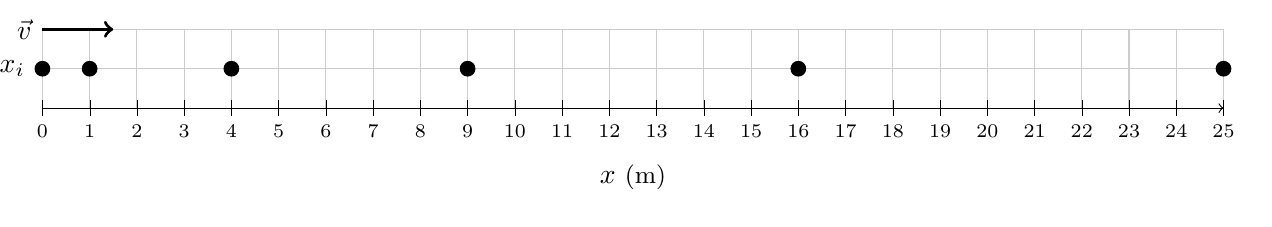
\begin{tikzpicture}[y=5mm,x=6mm]
    \draw[black!20,step=1] (0,0) grid (25,2);
        \foreach \x in {0,1,...,5}{
        \fill ({\x^2},1) circle (1mm);
    }
    \node[left=1mm,overlay] at (0,1) {$x_i$};
    \draw[very thick,->] (0,2) -- ++(1.5,0) node[left,pos=0,overlay] {$\vec{v}$};
    
    \foreach \x in {0,1,...,25} {
        \draw[ultra thin] (\x,-1mm) -- (\x,1mm) node[below=2mm] {\scriptsize $\x$};
    }
    \draw[->] (0,0) -- (25,0) node[below=6mm,pos=0.5] {$x$ {\small (m)}};
\end{tikzpicture}
\end{center}

\begin{parts}
\part Is the object speeding up or slowing down?

\begin{oneparchoices}
    \correctchoice speeding up
    \choice slowing down
\end{oneparchoices}

\part What is the direction of the object's acceleration? 

\begin{oneparchoices}
    \correctchoice rightward (positive)
    \choice leftward (negative)
\end{oneparchoices}
\end{parts}



\question % LG 1
The object below moves with negative velocity. 

\begin{center}
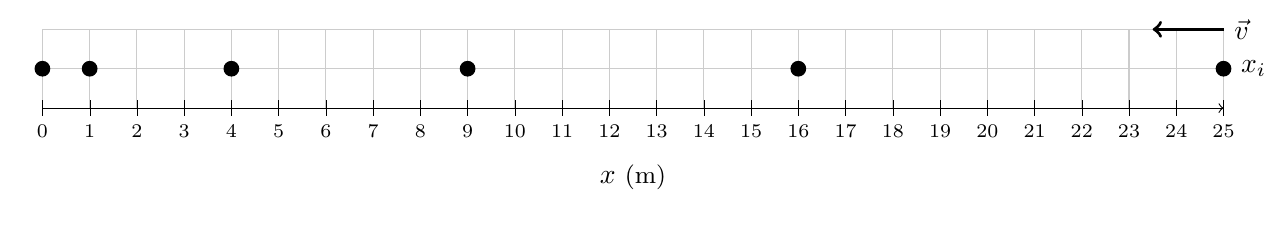
\begin{tikzpicture}[y=5mm,x=6mm]
    \draw[black!20,step=1] (0,0) grid (25,2);
        \foreach \x in {0,1,...,5}{
        \fill ({\x^2},1) circle (1mm);
    }
    \node[right=1mm,overlay] at (25,1) {$x_i$};
    \draw[very thick,->] (25,2) -- ++(-1.5,0) node[right,pos=0,overlay] {$\vec{v}$};
    
    \foreach \x in {0,1,...,25} {
        \draw[ultra thin] (\x,-1mm) -- (\x,1mm) node[below=2mm] {\scriptsize $\x$};
    }
    \draw[->] (0,0) -- (25,0) node[below=6mm,pos=0.5] {$x$ {\small (m)}};
\end{tikzpicture}
\end{center}

\begin{parts}
\part Is the object speeding up or slowing down?

\begin{oneparchoices}
    \choice speeding up
    \correctchoice slowing down
\end{oneparchoices}

\part What is the direction of the object's acceleration? 

\begin{oneparchoices}
    \correctchoice rightward (positive)
    \choice leftward (negative)
\end{oneparchoices}
\end{parts}


\question % LG 1
The object below moves with positive velocity. 

\begin{center}
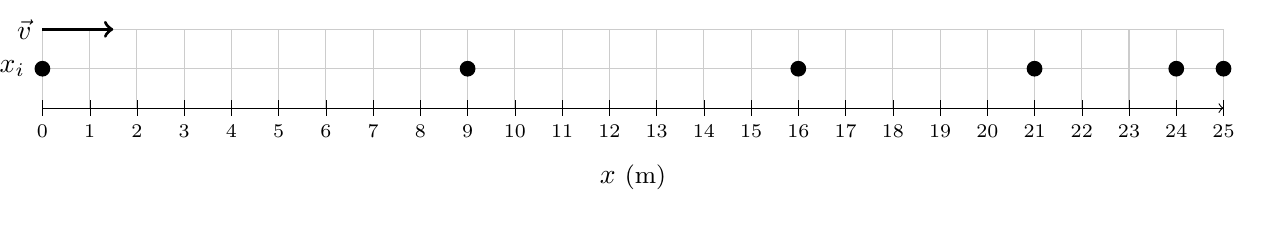
\begin{tikzpicture}[y=5mm,x=6mm]
    \draw[black!20,step=1] (0,0) grid (25,2);
    % Loop from 0 to 5 and subtract the square from 25
    \foreach \x in {0,1,...,5}{
        \fill ({25 - \x^2},1) circle (1mm);
    }
    \node[left=1mm,overlay] at (0,1) {$x_i$};
    
    \draw[very thick,->] (0,2) -- ++(1.5,0) node[left,pos=0,overlay] {$\vec{v}$};

    \foreach \x in {0,1,...,25} {
        \draw[ultra thin] (\x,-1mm) -- (\x,1mm) node[below=2mm] {\scriptsize $\x$};
    }
    \draw[->] (0,0) -- (25,0) node[below=6mm,pos=0.5] {$x$ {\small (m)}};
\end{tikzpicture}
\end{center}

\begin{parts}
\part Is the object speeding up or slowing down?

\begin{oneparchoices}
    \choice speeding up
    \correctchoice slowing down
\end{oneparchoices}

\part What is the direction of the object's acceleration? 

\begin{oneparchoices}
    \choice rightward (positive)
    \correctchoice leftward (negative)
\end{oneparchoices}
\end{parts}


\question % LG 1
The object below moves with negative velocity. 


\begin{center}
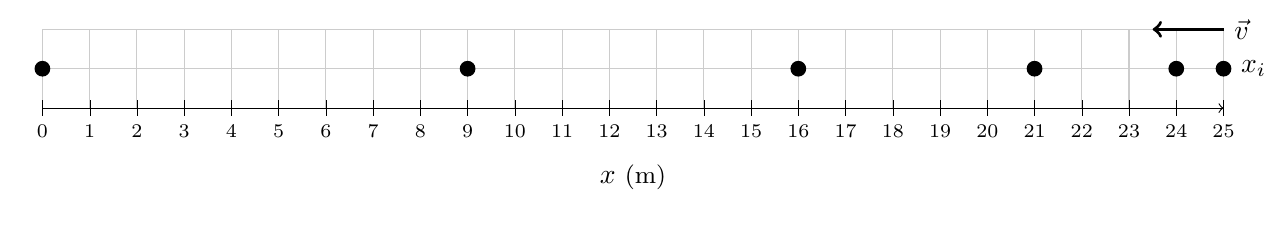
\begin{tikzpicture}[y=5mm,x=6mm]
    \draw[black!20,step=1] (0,0) grid (25,2);
    % Loop from 0 to 5 and subtract the square from 25
    \foreach \x in {0,1,...,5}{
        \fill ({25 - \x^2},1) circle (1mm);
    }
    \node[right=1mm,overlay] at (25,1) {$x_i$};
    \draw[very thick,->] (25,2) -- ++(-1.5,0) node[right,pos=0,overlay] {$\vec{v}$};

    \foreach \x in {0,1,...,25} {
        \draw[ultra thin] (\x,-1mm) -- (\x,1mm) node[below=2mm] {\scriptsize $\x$};
    }
    \draw[->] (0,0) -- (25,0) node[below=6mm,pos=0.5] {$x$ {\small (m)}};
\end{tikzpicture}
\end{center}

\begin{parts}
\part Is the object speeding up or slowing down?

\begin{oneparchoices}
    \correctchoice speeding up
    \choice slowing down
\end{oneparchoices}

\part What is the direction of the object's acceleration? 

\begin{oneparchoices}
    \choice rightward (positive)
    \correctchoice leftward (negative)
\end{oneparchoices}
\end{parts}

\end{questions}

\clearpage

\subsection*{LG 2 Practice}


\begin{questions}
\question \label{gqigC} % LG 2
  
\begin{minipage}[t]{8cm}
\vspace{-1.7ex}%

\begin{parts}
\part The object is\ldots

\begin{choices}
    \correctchoice speeding up.
    \choice slowing down.
    \choice speeding up, then slowing down.
    \choice slowing down, then speeding up.
    \choice not accelerating.
\end{choices}

\part The direction of acceleration is

\begin{choices}
    \correctchoice rightward (positive).
    \choice leftward (negative).
    \choice none (acceleration is zero).
\end{choices}
\end{parts}
\end{minipage}%
\begin{minipage}[t]{5cm}
\vspace{0pt}%
\centering


{\ifprintanswers \color{red} \else \color{white} \fi

\begin{equation*}
    v(t) = 2t
\end{equation*}
}

\vspace{-1em}

\def\arraystretch{1.5}
\velocitytableI{0}{2}{0}{1}
\end{minipage}

\question  % LG 2
  
\begin{minipage}[t]{8cm}
\vspace{-1.7ex}%

\begin{parts}
\part The object is\ldots

\begin{choices}
    \correctchoice speeding up.
    \choice slowing down.
    \choice speeding up, then slowing down.
    \choice slowing down, then speeding up.
    \choice not accelerating.
\end{choices}

\part The direction of acceleration is

\begin{choices}
    \choice rightward (positive).
    \correctchoice leftward (negative).
    \choice none (acceleration is zero).
\end{choices}
\end{parts}
\end{minipage}%
\begin{minipage}[t]{5cm}
\vspace{0em}%
\centering

{\ifprintanswers \color{red} \else \color{white} \fi

\begin{equation*}
    v(t) = -6 - 3t
\end{equation*}
}

\vspace{-1em}

\def\arraystretch{1.5}
\velocitytableI{-6}{-3}{0}{1}
\end{minipage}

\question % LG 2
  
\begin{minipage}[t]{8cm}
\vspace{-1.7ex}%

\begin{parts}
\part The object is\ldots

\begin{choices}
    \choice speeding up.
    \correctchoice slowing down.
    \choice speeding up, then slowing down.
    \choice slowing down, then speeding up.
    \choice not accelerating.
\end{choices}

\part The direction of acceleration is

\begin{choices}
    \choice rightward (positive).
    \correctchoice leftward (negative).
    \choice none (acceleration is zero).
\end{choices}
\end{parts}
\end{minipage}%
\begin{minipage}[t]{5cm}
\vspace{0em}%
\centering

{\ifprintanswers \color{red} \else \color{white} \fi

\begin{equation*}
    v(t) = 40 - 5t
\end{equation*}
}

\vspace{-1em}

\def\arraystretch{1.5}
\velocitytableI{40}{-5}{0}{2}
\end{minipage}

\question % LG 2
  
\begin{minipage}[t]{8cm}
\vspace{-1.7ex}%

\begin{parts}
\part The object is\ldots

\begin{choices}
    \choice speeding up.
    \correctchoice slowing down.
    \choice speeding up, then slowing down.
    \choice slowing down, then speeding up.
    \choice not accelerating.
\end{choices}

\part The direction of acceleration is

\begin{choices}
    \correctchoice rightward (positive).
    \choice leftward (negative).
    \choice none (acceleration is zero).
\end{choices}
\end{parts}
\end{minipage}%
\begin{minipage}[t]{5cm}
\vspace{0em}%
\centering

{\ifprintanswers \color{red} \else \color{white} \fi

\begin{equation*}
    v(t) = -9 + t
\end{equation*}
}

\vspace{-1em}

\def\arraystretch{1.5}
\velocitytableI{-9}{1}{0}{1}
\end{minipage}

\question % LG 2
  
\begin{minipage}[t]{8cm}
\vspace{-1.7ex}%

\begin{parts}
\part The object is\ldots

\begin{choices}
    \choice speeding up.
    \choice slowing down.
    \choice speeding up, then slowing down.
    \choice slowing down, then speeding up.
    \correctchoice not accelerating.
\end{choices}

\part The direction of acceleration is

\begin{choices}
    \choice rightward (positive).
    \choice leftward (negative).
    \correctchoice none (acceleration is zero).
\end{choices}
\end{parts}
\end{minipage}%
\begin{minipage}[t]{5cm}
\vspace{0em}%
\centering

{\ifprintanswers \color{red} \else \color{white} \fi

\begin{equation*}
    v(t) = 3
\end{equation*}
}

\def\arraystretch{1.5}
\velocitytableI{3}{0}{0}{1}
\end{minipage}

\question % LG 2
  
\begin{minipage}[t]{8cm}
\vspace{-1.7ex}%

\begin{parts}
\part The object is\ldots

\begin{choices}
    \choice speeding up.
    \choice slowing down.
    \choice speeding up, then slowing down.
    \correctchoice slowing down, then speeding up.
    \choice not accelerating.
\end{choices}

\part The direction of acceleration is

\begin{choices}
    \choice rightward (positive).
    \correctchoice leftward (negative).
    \choice none (acceleration is zero).
\end{choices}
\end{parts}
\end{minipage}%
\begin{minipage}[t]{5cm}
\vspace{0em}%
\centering
\def\arraystretch{1.5}

{\ifprintanswers \color{red} \else \color{white} \fi

\begin{equation*}
    v(t) = 8 - 4t
\end{equation*}
}

\velocitytableI{8}{-4}{0}{1}
\end{minipage}

\question % LG 2
  
\begin{minipage}[t]{8cm}
\vspace{-1.7ex}%

\begin{parts}
\part The object is\ldots

\begin{choices}
    \choice speeding up.
    \choice slowing down.
    \choice speeding up, then slowing down.
    \correctchoice slowing down, then speeding up.
    \choice not accelerating.
\end{choices}

\part The direction of acceleration is

\begin{choices}
    \correctchoice rightward (positive).
    \choice leftward (negative).
    \choice none (acceleration is zero).
\end{choices}
\end{parts}
\end{minipage}%
\begin{minipage}[t]{5cm}
\vspace{0em}%
\centering

{\ifprintanswers \color{red} \else \color{white} \fi

\begin{equation*}
    v(t) = -10 + 6t
\end{equation*}
}


\def\arraystretch{1.5}
\velocitytableI{-10}{6}{0}{1}
\end{minipage}




\end{questions}

\clearpage



\subsection*{LG 3 Practice}

% \textbf{Questions \ref{bkoxL}--\ref{SGatV}.} Identify whether or not the object in the table is accelerating, and state whether the acceleration is positive, negative, or zero.

\begin{questions}

\question \label{bkoxL} % LG 3

\begin{minipage}[t]{8cm}
\vspace{-1.7ex}%

\begin{parts}
\part The object is\ldots

\begin{choices}
    \correctchoice speeding up.
    \choice slowing down.
    \choice speeding up, then slowing down.
    \choice slowing down, then speeding up.
    \choice not accelerating.
\end{choices}


\part The direction of acceleration is

\begin{choices}
    \correctchoice rightward (positive).
    \choice leftward (negative).
    \choice none (acceleration is zero).
\end{choices}
\end{parts}
\end{minipage}%
\begin{minipage}[t]{5cm}
\vspace{0em}%
\centering

{\ifprintanswers \color{red} \else \color{white} \fi

\begin{align*}
    v(t) &= 2t \\[1ex]
    x(t) &= t^2
\end{align*}
}

\vspace{-1em}

\def\arraystretch{1.5}
\positiontableI{0}{0}{0}{1}{2}
\end{minipage}

\question \label{bkoxL} % LG 3

\begin{minipage}[t]{8cm}
\vspace{-1.7ex}%

\begin{parts}
\part The object is\ldots

\begin{choices}
    \correctchoice speeding up.
    \choice slowing down.
    \choice speeding up, then slowing down.
    \choice slowing down, then speeding up.
    \choice not accelerating.
\end{choices}


\part The direction of acceleration is

\begin{choices}
    \choice rightward (positive).
    \correctchoice leftward (negative).
    \choice none (acceleration is zero).
\end{choices}
\end{parts}
\end{minipage}%
\begin{minipage}[t]{5cm}
\vspace{0em}%
\centering

{\ifprintanswers \color{red} \else \color{white} \fi

\begin{align*}
    v(t) &= -6 - 3t \\
    x(t) &= 48 - 6t -\frac{3}{2}t^2
\end{align*}
}

\vspace{-1ex}

\def\arraystretch{1.5}
\positiontableI{48}{-6}{0}{2}{-3}
\end{minipage}

\question % LG 3

\begin{minipage}[t]{8cm}
\vspace{-1.7ex}%

\begin{parts}
\part The object is\ldots

\begin{choices}
    \choice speeding up.
    \correctchoice slowing down.
    \choice speeding up, then slowing down.
    \choice slowing down, then speeding up.
    \choice not accelerating.
\end{choices}


\part The direction of acceleration is

\begin{choices}
    \choice rightward (positive).
    \correctchoice leftward (negative).
    \choice none (acceleration is zero).
\end{choices}
\end{parts}
\end{minipage}%
\begin{minipage}[t]{5cm}
\vspace{0em}%
\centering

{\ifprintanswers \color{red} \else \color{white} \fi

\begin{align*}
    v(t) &= 40 - 5t \\
    x(t) &= -80 + 40t - \frac{5}{2}t^2
\end{align*}
}

\vspace{-1ex}

\def\arraystretch{1.5}
\positiontableI{-80}{40}{0}{2}{-5}
\end{minipage}

\question % LG 3

\begin{minipage}[t]{8cm}
\vspace{-1.7ex}%

\begin{parts}
\part The object is\ldots

\begin{choices}
    \choice speeding up.
    \correctchoice slowing down.
    \choice speeding up, then slowing down.
    \choice slowing down, then speeding up.
    \choice not accelerating.
\end{choices}


\part The direction of acceleration is

\begin{choices}
    \correctchoice rightward (positive).
    \choice leftward (negative).
    \choice none (acceleration is zero).
\end{choices}
\end{parts}
\end{minipage}%
\begin{minipage}[t]{5cm}
\vspace{-1ex}%
\centering

{\ifprintanswers \color{red} \else \color{white} \fi

\begin{align*}
    v(t) &= -9 + t \\
    x(t) &= 48 - 9t + \frac{1}{2}t^2
\end{align*}
}

\vspace{-1ex}

\def\arraystretch{1.5}
\positiontableI{48}{-9}{0}{2}{1}
\end{minipage}

\question % LG 3

\begin{minipage}[t]{8cm}
\vspace{-1.7ex}%

\begin{parts}
\part The object is\ldots

\begin{choices}
    \choice speeding up.
    \choice slowing down.
    \choice speeding up, then slowing down.
    \choice slowing down, then speeding up.
    \correctchoice not accelerating.
\end{choices}

\part The direction of acceleration is

\begin{choices}
    \choice rightward (positive).
    \choice leftward (negative).
    \correctchoice none (acceleration is zero).
\end{choices}
\end{parts}
\end{minipage}%
\begin{minipage}[t]{5cm}
\vspace{-1ex}%
\centering

{\ifprintanswers \color{red} \else \color{white} \fi

\begin{align*}
    v(t) &= 3 \\[1ex]
    x(t) &= 3t   
\end{align*}
}

\vspace{-1em}

\def\arraystretch{1.5}
\positiontableI{0}{3}{0}{1}{0}
\end{minipage}

\question  % LG 3

\begin{minipage}[t]{8cm}
\vspace{-1.7ex}%

\begin{parts}
\part The object is\ldots

\begin{choices}
    \choice speeding up.
    \choice slowing down.
    \choice speeding up, then slowing down.
    \correctchoice slowing down, then speeding up.
    \choice not accelerating.
\end{choices}

\part The direction of acceleration is

\begin{choices}
    \choice rightward (positive).
    \correctchoice leftward (negative).
    \choice none (acceleration is zero).
\end{choices}
\end{parts}
\end{minipage}%
\begin{minipage}[t]{5cm}
\vspace{-1ex}%
\centering

{\ifprintanswers \color{red} \else \color{white} \fi

\begin{align*}  
    v(t) &= 8 - 4t \\[1ex]
    x(t) &= 8t - 2t^2
\end{align*}
}

\vspace{-1em}

\def\arraystretch{1.5}
\positiontableI{0}{8}{0}{1}{-4}
\end{minipage}

\question  % LG 3

\begin{minipage}[t]{8cm}
\vspace{-1.7ex}%

\begin{parts}
\part The object is\ldots

\begin{choices}
    \choice speeding up.
    \choice slowing down.
    \choice speeding up, then slowing down.
    \correctchoice slowing down, then speeding up.
    \choice not accelerating.
\end{choices}

\part The direction of acceleration is

\begin{choices}
    \correctchoice rightward (positive).
    \choice leftward (negative).
    \choice none (acceleration is zero).
\end{choices}
\end{parts}
\end{minipage}%
\begin{minipage}[t]{5cm}
\vspace{-1ex}%
\centering

{\ifprintanswers \color{red} \else \color{white} \fi

\begin{align*}  
    v(t) &= -10 + 6t \\[1ex]
    x(t) &= 12 -10t - 3t^2
\end{align*}
}

\vspace{-1em}

\def\arraystretch{1.5}
\positiontableI{12}{-10}{0}{1}{6}
\end{minipage}









\end{questions}

\clearpage




\subsection*{LG 4,5 Practice}

\textbf{Questions.} Determine whether or not each of the following graphs represents accelerating motion.

\begin{questions}
\begin{multicols}{2}

\question %...LG 5 H
Accelerating? Yes or No?

\positiongraphII{1}{1}{-1}

\ifprintanswers 
\textcolor{red}{Yes, accelerating. Position is changing quadratically with time.}
\else \textit{Reasoning:} \fillin[][0.73\linewidth]
\fillwithlines{7mm}
\fi

\question %...LG 4 C
Accelerating? Yes or No?

\velocitygraphI{-2}{2}

\ifprintanswers 
\textcolor{red}{Yes, accelerating. Velocity is changing linearly with time.}
\else \textit{Reasoning:} \fillin[][0.73\linewidth]
\fillwithlines{7mm}
\fi


\question \label{IMwAV} %...LG 5 L
Accelerating? Yes or No?

\positiongraphII{3}{-2}{0}

\ifprintanswers 
\textcolor{red}{No, not accelerating. Since position is changing linearly with time, the velocity must be constant ($a = 0$).}
\else \textit{Reasoning:} \fillin[][0.73\linewidth]
\fillwithlines{7mm}
\fi


\vspace*{\fill}
\columnbreak

\question %...LG 4 A
Accelerating? Yes or No?

\velocitygraphI{0}{-6}

\ifprintanswers \else \textit{Reasoning:} \fillin[][0.73\linewidth]
\fillwithlines{7mm}
\fi

\question %...LG 4 F
Accelerating? Yes or No?

\velocitygraphI{1.8}{-5}

\ifprintanswers \else \textit{Reasoning:} \fillin[][0.73\linewidth]
\fillwithlines{7mm}
\fi

\question %...LG 5 J
Accelerating? Yes or No?

\positiongraphII{0}{4}{-2}

\ifprintanswers \else \textit{Reasoning:} \fillin[][0.73\linewidth]
\fillwithlines{7mm}
\fi

\clearpage

\question %...LG 4 D
Accelerating? Yes or No?

\velocitygraphI{0}{3}

\ifprintanswers \else \textit{Reasoning:} \fillin[][0.73\linewidth]
\fillwithlines{7mm}
\fi

\question %...LG 5 K
Accelerating? Yes or No?

\positiongraphII{2}{-6}{2.5}

\ifprintanswers \else \textit{Reasoning:} \fillin[][0.73\linewidth]
\fillwithlines{7mm}
\fi

\question %...LG 4 B
Accelerating? Yes or No?

\velocitygraphI{1}{0}

\ifprintanswers \else \textit{Reasoning:} \fillin[][0.73\linewidth]
\fillwithlines{7mm}
\fi

\question %...LG 5 I
Accelerating? Yes or No?

\positiongraphII{0}{1}{0}

\ifprintanswers \else \textit{Reasoning:} \fillin[][0.73\linewidth]
\fillwithlines{7mm}
\fi

\question \label{H2UaC} %...LG 5 G
Accelerating? Yes or No?

\positiongraphII{-1}{-1}{1}

\ifprintanswers \else \textit{Reasoning:} \fillin[][0.73\linewidth]
\fillwithlines{7mm}
\fi

\question %...LG 4 E
Accelerating? Yes or No?

\velocitygraphI{-0.1}{6}

\ifprintanswers \else \textit{Reasoning:} \fillin[][0.73\linewidth]
\fillwithlines{7mm}
\fi



% \end{multicols}
% \end{questions}


% \clearpage

% \subsection*{LG 5 Practice}

% \textbf{Questions \ref{H2UaC}--\ref{IMwAV}.} Indicate whether or not the following objects are accelerating based on the position vs.\,time graph. Justify your answer.

% \begin{questions}
% \begin{multicols}{2}













\end{multicols}
\end{questions}

\clearpage

\subsection*{LG 6 Practice}

For each velocity-vs-time graph below, determine the direction (right or left) of the object. If there's no acceleration, write ``not accelerating.''


\begin{questions}
\begin{multicols}{2}

\question
\textit{Direction of acceleration:} \fillin[][3cm]

\velocitygraphII{-4}{1}

    

\question
\textit{Direction of acceleration:} \fillin[][3cm]

\velocitygraphII{3}{-1.5}


\question
\textit{Direction of acceleration:} \fillin[][3cm]

\velocitygraphII{-3}{1.5}

\question
\textit{Direction of acceleration:} \fillin[][3cm]

\velocitygraphII{2}{0}

\vspace*{\fill}
\columnbreak



\question \textit{Direction of acceleration:} \fillin[leftward][3cm]
\velocitygraphII{4}{-1}

\question
\textit{Direction of acceleration:} \fillin[][3cm]

\velocitygraphII{-2}{0}

\question
\textit{Direction of acceleration:} \fillin[][3cm]

\velocitygraphII{3}{-0.15}

\question
\textit{Direction of acceleration:} \fillin[][3cm]

\velocitygraphII{-2}{0.1}





\end{multicols}
\end{questions}



\clearpage

\subsection*{Review LG 1--6}

\begin{questions}
\question
Fill in the table below.
\vspace{-1em}

\begin{EnvUplevel}
\def\arraystretch{1.5}
\begin{center}
\begin{tabular}{|w{c}{1cm}|w{c}{4cm}||w{c}{5cm}|w{c}{1.5cm}||w{c}{2cm}|}
    \hline
    \thead{\bfseries Symbol} & \thead{\bfseries Quantity} & \thead{\bfseries SI Unit} & \thead{\bfseries Unit\\ \bfseries Symbol} & \thead{\bfseries Example}\\ \hline
    $x$ & \ans{position} & meters & m & $x = \SI{5}{m}$ \\ \hline 
    $\Delta t$ & (change in) time & \ans{seconds} & s & \ans{$\Delta t = \SI{45}{s}$} \\ \hline 
    \ans{$v$} & \ans{velocity} & meters per second & \ans{m/s} & \ans{$v = -\SI{4}{m/s}$} \\ \hline 
    $a$ & \ans{acceleration} & meters per second squared & \ans{\SI{}{m/s^2}} & \ans{$a = +\SI{3}{m/s^2}$} \\ \hline 
\end{tabular}
\end{center}
\end{EnvUplevel}



\question 
The number that shows an object's location on a horizontal track is called the \fillin[position][3cm].

\begin{center}
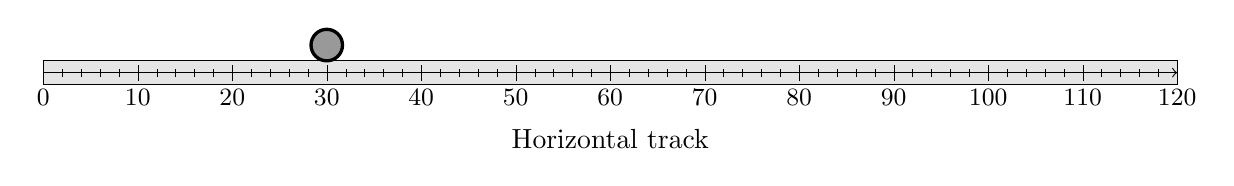
\begin{tikzpicture}[x=1.2mm]
    \draw[fill=black!10] (0,-1.5mm) rectangle (120,1.5mm);
    \foreach \x in {0,10,...,120} {
        \draw[ultra thin] (\x,-1mm) -- (\x,1mm) node[below=2mm] {\small $\x$};
    }
    \foreach \x in {0,2,...,120} {
        \draw[ultra thin] (\x,-0.5mm) -- (\x,0.5mm);
    }
    \draw[->] (0,0) -- (120,0) node[below=6mm,pos=0.5] {Horizontal track};
    \draw[very thick,fill=black!40] (30,3.5mm) circle (2mm);
\end{tikzpicture} 
\end{center}


\question 
Velocity is the rate at which \fillin[position][3cm]\ changes with time.

\question
Acceleration is the rate at which \fillin[velocity][3cm]\ changes with time.

\question
Label 2 points below as $\left(x_1,y_1\right)$ and $\left(x_2,y_2\right)$. Then, find the slope of the line. Show all your work. 

\begin{EnvUplevel}
\centering

\begin{minipage}[t]{8cm}
\vspace{0pt}%
\centering
\begin{tikzpicture}
    \begin{axis}[height=6.2cm,width=7cm,
        axis y line=left,
        axis x line = center,
        ylabel={$y$},
        xlabel={$x$},
        ylabel style ={rotate=-90,at={(axis description cs:-0.1,0.9)}},
        ymin=-4,ymax=4,
        xmin=0,xmax=8,
        ytick={-4,-3,...,4},
        xtick={0,1,...,8},
        grid=both, 
        % minor y tick num=1,
        % minor x tick num=1,
    ]
        \addplot[very thick,domain=1:6] {2*x-7};
        \ifprintanswers
        \fill[red] (2,-3) circle (3pt);
        \fill[red] (5,3) circle (3pt);
        \node[red,align=center,right=2mm] at (2,-3) {$(x_1,y_1)$\\[1ex]$(2,-3)$};
        \node[red,align=left,shift={(8mm,-1mm)}] at (5,3) {$(x_2,y_2)$\\[1ex]$(5,3)$};
        \fi
    \end{axis}
\end{tikzpicture}
\end{minipage}%
\fbox{
\begin{minipage}[t]{7.5cm}
\vspace{0pt}%
\centering
\vspace{1ex}
{\ifprintanswers \color{red} \else \color{white} \fi
\begin{align*}
    \text{slope} = m &= \mathrm{\frac{rise}{run}} \\[1ex]
    &= \frac{y_2 - y_1}{x_2 - x_1} \\[1ex]
    &= \frac{3 - (-3)}{5 - 2} \\[1ex]
    &= \frac{6}{3} \\[1ex]
    &= \boxed{2}
\end{align*}
}
\vspace{-1em}
\end{minipage}}
\end{EnvUplevel}

\question
Each box below shows a steel ball's velocity vector. Below this vector, draw an acceleration vector that matches the description below the box of the ball's change in speed.

\begin{EnvUplevel}
\centering
\begin{minipage}{3.5cm}
\centering
\begin{tikzpicture}
    \draw (0,0) rectangle (3,2);
    \draw[line width=1mm,-{Triangle[scale=1]}] (0.5,1.5) -- ++(2,0) node[above,pos=0.5] {$v$};
    {\ifprintanswers \color{red} \else \color{white} \fi
    \draw[line width=1mm,-{Triangle[scale=1]}] (0.5,0.5) -- ++(2,0) node[above,pos=0.5] {$a$};}
    \node[below] at (current bounding box.south) {speeding up};
\end{tikzpicture}
\end{minipage}%
\begin{minipage}{3.5cm}
\centering
\begin{tikzpicture}
    \draw (0,0) rectangle (3,2);
    \draw[line width=1mm,-{Triangle[scale=1]}] (0.5,1.5) -- ++(2,0) node[above,pos=0.5] {$v$};
    {\ifprintanswers \color{red} \else \color{white} \fi
    \draw[line width=1mm,{Triangle[scale=1]}-] (0.5,0.5) -- ++(2,0) node[above,pos=0.5] {$a$};}
    \node[below] at (current bounding box.south) {slowing down};
\end{tikzpicture}
\end{minipage}%
\begin{minipage}{3.5cm}
\centering
\begin{tikzpicture}
    \draw (0,0) rectangle (3,2);
    \draw[line width=1mm,{Triangle[scale=1]}-] (0.5,1.5) -- ++(2,0) node[above,pos=0.5] {$v$};
    {\ifprintanswers \color{red} \else \color{white} \fi
    \draw[line width=1mm,{Triangle[scale=1]}-] (0.5,0.5) -- ++(2,0) node[above,pos=0.5] {$a$};}
    \node[below] at (current bounding box.south) {speeding up};
\end{tikzpicture}
\end{minipage}%
\begin{minipage}{3.5cm}
\centering
\begin{tikzpicture}
    \draw (0,0) rectangle (3,2);
    \draw[line width=1mm,{Triangle[scale=1]}-] (0.5,1.5) -- ++(2,0) node[above,pos=0.5] {$v$};
    {\ifprintanswers \color{red} \else \color{white} \fi
    \draw[line width=1mm,-{Triangle[scale=1]}] (0.5,0.5) -- ++(2,0) node[above,pos=0.5] {$a$};}
    \node[below] at (current bounding box.south) {slowing down};
\end{tikzpicture}
\end{minipage}%
\end{EnvUplevel}

\question
When an object's velocity and acceleration are in \underline{opposite} directions, the object \fillin[slows down][3cm].\\[1em]
When an object's velocity and acceleration are in the \underline{same} direction, the object \fillin[speeds up][3cm].

\clearpage

\question
Create a velocity table for an object undergoing constant acceleration.

\begin{minipage}[t]{5cm}
\vspace{0pt}%
\def\arraystretch{1.3}
\begin{tabular}{|c|c|}
    \hline
    \thead{\bfseries Time (s)} & \thead{\bfseries Velocity (m/s)} \\ \hline
    0 & \ans{0} \\ \hline
    1 & \ans{2} \\ \hline
    2 & \ans{4} \\ \hline
    3 & \ans{6} \\ \hline
    4 & \ans{8} \\ \hline
    5 & \ans{10} \\ \hline
\end{tabular}
\end{minipage}%
\begin{minipage}[t]{10cm}
\vspace{0pt}%
\begin{parts}
\part In your own words, what does acceleration mean?

\ifprintanswers
\textcolor{red}{Acceleration is the rate at which velocity changes with time.}
\else 
\fillwithlines{14mm}
\fi

\part Why does your table represent acceleration?

\ifprintanswers
\textcolor{red}{The velocities are not constant but changing with time.}
\else 
\fillwithlines{14mm}
\fi
\end{parts}
\end{minipage}

\question
\begin{parts}
\part Using the table, graph position vs time.

\begin{center}
\begin{minipage}[t]{3cm}
\vspace{0pt}%
\def\arraystretch{2}
\begin{tabular}{|c|c|}
    \hline
    \thead{$t$ (s)} & \thead{$x$ (m)} \\ \hline
    0 & 0 \\ \hline
    1 & 1 \\ \hline
    2 & 4 \\ \hline
    3 & 9 \\ \hline
    4 & 16 \\ \hline
    5 & 25 \\ \hline
\end{tabular}
\end{minipage}%
\begin{minipage}[t]{10cm}
\vspace{0pt}%
\centering
\begin{tikzpicture}
    \begin{axis}[height=7cm,width=9cm,
        ylabel={\small Position (m)},
        xlabel={\small Time (s)},
        ymin=0,ymax=25,
        xmin=0,xmax=5,
        ytick={0,5,...,25},
        xtick={0,1,...,5},
        grid=both,
        axis lines=left,
        clip=false,
        major grid style={thick, draw=black!60},
        minor grid style={thin, draw=gray!30},
        minor y tick num=4,
        minor x tick num=4,
    ]
        \ifprintanswers
            \addplot[only marks,mark=*,red] coordinates{(0,0)(1,1)(2,4)(3,9)(4,16)(5,25)};
            \addplot[red,smooth,domain=0:5,thick] {x^2}; 
        \fi
    \end{axis}
\end{tikzpicture}
\end{minipage}
\end{center}

\part What is the shape of this $x$ vs $t$ graph?\ \fillin[quadratic][4cm]
\end{parts}



\question
\begin{parts}
\part In the velocity vs time graphs below, indicate the direction (leftward/rightward) of acceleration.
\vspace{-1ex}

\begin{EnvUplevel}
\centering
\fbox{
\begin{minipage}[t]{3cm}
\vspace{0pt}%
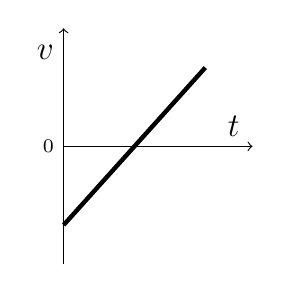
\begin{tikzpicture}[y=2.5cm,x=2cm]
    \draw[->] (0,0) -- (1.2,0) node[above,pos=0.9] {\large $t$} node[left,pos=0] {\scriptsize 0};
    \draw[->] (0,-0.6) -- (0,0.6) node[left,pos=0.9] {\large $v$};
    \draw[ultra thick] (0,-0.4) -- (0.9,0.4);
\end{tikzpicture}
\end{minipage}%
\begin{minipage}[t]{4.5cm}
\vspace{7mm}%
\raggedleft
\begin{tikzpicture}
    \node[above] at (0,0) {positive slope};
    \draw[line width=1mm,-{Triangle[scale=0.5]}] (0,0) -- ++(0,-0.5);
    \node[below] at (0,-0.5) {\fillin[rightward][2.2cm] acceleration};
\end{tikzpicture}
\end{minipage}}%
\hspace{5mm}
\fbox{
\begin{minipage}[t]{3cm}
\vspace{0pt}%
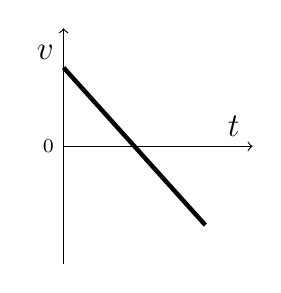
\begin{tikzpicture}[y=2.5cm,x=2cm]
    \draw[->] (0,0) -- (1.2,0) node[above,pos=0.9] {\large $t$} node[left,pos=0] {\scriptsize 0};
    \draw[->] (0,-0.6) -- (0,0.6) node[left,pos=0.9] {\large $v$};
    \draw[ultra thick] (0,0.4) -- (0.9,-0.4);
\end{tikzpicture}
\end{minipage}%
\begin{minipage}[t]{4.5cm}
\vspace{7mm}%
\raggedleft
\begin{tikzpicture}
    \node[above] at (0,0) {negative slope};
    \draw[line width=1mm,-{Triangle[scale=0.5]}] (0,0) -- ++(0,-0.5);
    \node[below] at (0,-0.5) {\fillin[leftward][2.2cm] acceleration};
\end{tikzpicture}
\end{minipage}}%
\end{EnvUplevel}

\vspace{1em}

\part For the position vs time graphs below, fill in the blanks using words from the following list: 
\vspace{1ex}

\begin{center}
\bfseries
acceleration,\quad constant,\quad linear,\quad quadratic,\quad velocity,\quad zero
\end{center}

\begin{EnvUplevel}
\centering
\fbox{
\begin{minipage}[t]{3cm}
\vspace{0pt}%
\centering
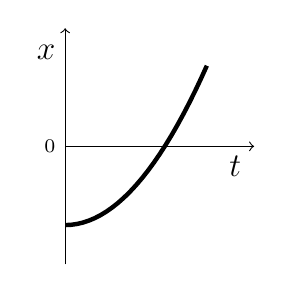
\begin{tikzpicture}[y=2.5cm,x=2cm]
    \draw[->] (0,0) -- (1.2,0) node[below,pos=0.9] {\large $t$} node[left,pos=0] {\scriptsize 0};
    \draw[->] (0,-0.6) -- (0,0.6) node[left,pos=0.9] {\large $x$};
    \draw[ultra thick,domain=0:0.9] plot({\x},{\x^2-0.4});
\end{tikzpicture}
\end{minipage}%
\begin{minipage}[t]{4.5cm}
\vspace{5mm}%
\raggedleft
\fillin[quadratic]\ shape\, \\[1em]
changing \fillin[velocity]\,  \\[1em]
constant \fillin[acceleration]\, 
\end{minipage}}%
\hspace{5mm}
\fbox{
\begin{minipage}[t]{3cm}
\vspace{0pt}%
\centering
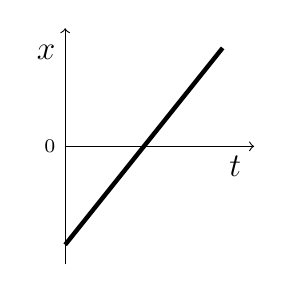
\begin{tikzpicture}[y=2.5cm,x=2cm]
    \draw[->] (0,0) -- (1.2,0) node[below,pos=0.9] {\large $t$} node[left,pos=0] {\scriptsize 0};
    \draw[->] (0,-0.6) -- (0,0.6) node[left,pos=0.9] {\large $x$};
    \draw[ultra thick] (0,-0.5) -- (1,0.5);
\end{tikzpicture}
\end{minipage}%
\begin{minipage}[t]{4.5cm}
\vspace{5mm}%
\raggedleft
\fillin[linear]\ shape\, \\[1em]
\fillin[constant]\ velocity \\[1em]
\fillin[zero][2cm]\ acceleration
\end{minipage}}%
\end{EnvUplevel}
\end{parts}

\end{questions}
\clearpage


\subsection*{LG 7 Practice}

% \textbf{Questions \ref{jpyYo}--\ref{OK5PY}.} For each of the following questions, at the specified point, (a) draw the tangent line to the curve at the given point, (b) state whether the object is on the right side or left side of the origin, and (c) determine the direction of the object's velocity at that point.


The figure below shows an object on the right side of the origin, moving with leftward velocity.

\begin{center}
\begin{tikzpicture}[x=1.2cm]
    \foreach \x in {-4,-3,...,4} {
        \draw[ultra thin] (\x,-1mm) -- (\x,1mm) node[below=2mm] {$\x$};
    }
    \draw[->] (-4,0) -- (4,0) node[pos=0.5,below=5mm] {$x = \text{Position (m)}$};
    \node at (3,0.32) {\resizebox{1cm}{!}{\usym{1F699}}};
    \draw[line width=1mm,-{Triangle[scale=0.7]}] (0,0.8) -- (0,0.2) node[above,pos=0] {origin};
    \draw[very thick,->] (2.5,0.5) -- ++(-0.6,0) node[above,pos=0.5] {$\vec{v}$};
    \speedometer{(5,0.5)}{60}{12}
\end{tikzpicture}
\end{center}

\noindent The motion of such object could be represented by all of the position vs time graphs in the questions below. For each question:

\begin{itemize}[topsep=0pt,itemsep=0pt]
    \item Draw the tangent line to the curve at the point shown.
    \item Identify the direction of the object's position vector at the point. (What is the  direction of location relative to the origin?)
    \item Identify the direction of the object's velocity at the point. (In what direction is the object moving?)
\end{itemize}

\begin{questions}

\begin{multicols}{2} % Start 2-column layout

\question \label{jpyYo}
\begin{parts}
\part Draw the tangent line to curve at the specified point.
\part At the point, the object is on the \fillin[left][3cm]\ side of the origin.
\part At the point, the object's velocity vector points to the \fillin[right][3cm].
\vspace{1em}

\begin{tikzpicture}[x=3cm,y=2cm,
        declare function={
                f(\t)  = -(\t-0.8)^2;
                df(\t) = -2*(\t-0.8);
            }
    ]
    
    \draw[->] (0,-1) -- (0,1) node[left,pos=0.95] {\large $x$} node[pos=0.5,left] {\footnotesize $0$};
    \draw[->] (0,0) -- (1,0) node[right] {\large $t$};
    \draw[very thick,domain=0:0.8,smooth,variable=\t] plot(\t,{f(\t)});

    % % 1. Define your tangent point t_0 here
    \pgfmathsetmacro{\tzero}{0.3}
    
    % 2. The Point (automatically calculated)
    \fill (\tzero,{f(\tzero}) circle (2.5pt);
    
    % 3. Tangent Line using the raw point-slope formula: x = m*(t - t_0) + x_0  
    \ifprintanswers
        \draw[thick,red,domain=-0.2:1,variable=\t] plot(\t, {df(\tzero)*(\t-\tzero) + f(\tzero});
    \fi
\end{tikzpicture}
\end{parts}



% \ifprintanswers
% \textcolor{red}{(b) The object is on the left side of the origin, since the position $x$ is negative.\\ (c) The direction of the object's velocity is to the right, because the slope of the tangent line is positive.}
% \fi

\question
\begin{parts}
\part Draw the tangent line to curve at the specified point.
\part At the point, the object is on the \fillin[right][3cm]\ side of the origin.
\part At the point, the object's velocity vector points to the \fillin[left][3cm].
\vspace{1em}

\begin{tikzpicture}[x=3cm,y=2cm,
        declare function={
                f(\t)  = (\t-0.8)^2;
                df(\t) = 2*(\tzero-0.8);
            }
    ]
    
    \draw[->] (0,-1) -- (0,1) node[left,pos=0.95] {\large $x$} node[pos=0.5,left] {\footnotesize $0$};
    \draw[->] (0,0) -- (1,0) node[right] {$t$};
    \draw[very thick,domain=0:0.8,smooth,variable=\t] plot(\t,{f(\t)});

    % 1. Define your tangent point t_0 here
    \pgfmathsetmacro{\tzero}{0.3}

    % 2. The Point (automatically calculated)
    \fill (\tzero,{f(\tzero)}) circle (2.5pt);

    % 3. Tangent Line using the raw point-slope formula: x = m*(t - t_0) + x_0  
    \ifprintanswers
        \draw[thick,red,domain=-0.2:1,variable=\t] plot(\t, {df(\tzero)*(\t-\tzero) + f(\tzero)}); 
    \fi
\end{tikzpicture}
\end{parts}

\vspace*{\fill}
\columnbreak

\question
\begin{parts}
\part Draw the tangent line to curve at the specified point.
\part At the point, the object is on the \fillin[left][3cm]\ side of the origin.
\part At the point, the object's velocity vector points to the \fillin[left][3cm].
\vspace{1em}

\begin{tikzpicture}[x=3cm,y=2cm,
        declare function={
                f(\t)  = -\t^2;
                df(\t) = -2*\t;
            }
    ]

    \draw[->] (0,-1) -- (0,1) node[left,pos=0.95] {\large $x$} node[pos=0.5,left] {\footnotesize $0$};
    \draw[->] (0,0) -- (1,0) node[right] {$t$};
    \draw[very thick,domain=0:0.8,smooth,variable=\t] plot(\t,{f(\t)});

    % 1. Define your tangent point t_0 here
     \pgfmathsetmacro{\tzero}{0.5}

    % 2. The Point (automatically calculated)
    \fill (\tzero,{f(\tzero)}) circle (2.5pt);

    % 3. Tangent Line using the raw point-slope formula: x = m*(t - t_0) + x_0  
    \ifprintanswers
        \draw[thick,red,domain=-0.2:1,variable=\t] plot(\t, {df(\tzero)*(\t-\tzero) + f(\tzero)}); 
    \fi
\end{tikzpicture}
\end{parts}



\question
\begin{parts}
\part Draw the tangent line to curve at the specified point.
\part At the point, the object is on the \fillin[right][3cm]\ side of the origin.
\part At the point, the object's velocity vector points to the \fillin[right][3cm].
\vspace{1em}

\begin{tikzpicture}[x=3cm,y=2cm,
        declare function={
                f(\t)  = \t^2;
                df(\t) = 2*\t;
            }
    ]
    
    \draw[->] (0,-1) -- (0,1) node[left,pos=0.95] {\large $x$} node[pos=0.5,left] {\footnotesize $0$};
    \draw[->] (0,0) -- (1,0) node[right] {$t$};
    \draw[very thick,domain=0:0.8,smooth,variable=\t] plot(\t,{f(\t)});

    % 1. Define your tangent point t_0 here
    \pgfmathsetmacro{\tzero}{0.5}

    % 2. The Point (automatically calculated)
    \fill (\tzero,{f(\tzero)}) circle (2.5pt);

    % 3. Tangent Line using the raw point-slope formula: x = m*(t - t_0) + x_0  
    \ifprintanswers
        \draw[thick,red,domain=-0.2:1,variable=\t]  plot(\t, {df(\tzero)*(\t-\tzero) + f(\tzero)}); 
    \fi
\end{tikzpicture}
\end{parts}

\vspace*{\fill}
\columnbreak

\question
\begin{parts}
\part Draw the tangent line to curve at the specified point.
\part At the point, the object is on the \fillin[right][3cm]\ side of the origin.
\part At the point, the object's velocity vector points to the \fillin[right][3cm].
\vspace{1em}

\begin{tikzpicture}[x=3cm,y=2cm,
        declare function={
                f(\t)  = -(\t - 0.8)^2 + 0.8^2;
                df(\t) = -2*(\t - 0.8);
            }
    ]
    
    \draw[->] (0,-1) -- (0,1) node[left,pos=0.95] {\large $x$} node[pos=0.5,left] {\footnotesize $0$};
    \draw[->] (0,0) -- (1,0) node[right] {$t$};
    \draw[very thick,domain=0:0.8,smooth,variable=\t] plot(\t,{f(\t)});

    % 1. Define your tangent point t_0 here
    \pgfmathsetmacro{\tzero}{0.4}

    % 2. The Point (automatically calculated)
    \fill (\tzero,{f(\tzero)}) circle (2.5pt);

    % 3. Tangent Line using the raw point-slope formula: x = m*(t - t_0) + x_0  
    \ifprintanswers
        \draw[thick,red,domain=-0.2:1,variable=\t] plot(\t, {df(\tzero)*(\t - \tzero) + f(\tzero)});
    \fi
\end{tikzpicture}
\end{parts}

\question
\begin{parts}
\part Draw the tangent line to curve at the specified point.
\part At the point, the object is on the \fillin[left][3cm]\ side of the origin.
\part At the point, the object's velocity vector points to the \fillin[left][3cm].
\vspace{1em}

\begin{tikzpicture}[x=3cm,y=2cm,
        declare function={
                f(\t)  = (\t - 0.8)^2 - 0.8^2;
                df(\t) = 2*(\t - 0.8);
            }
    ]
    
    \draw[->] (0,-1) -- (0,1) node[left,pos=0.95] {\large $x$} node[pos=0.5,left] {\footnotesize $0$};
    \draw[->] (0,0) -- (1,0) node[right] {$t$};
    \draw[very thick,domain=0:0.8,smooth,variable=\t] plot(\t,{f(\t)});

    % 1. Define your tangent point t_0 here
    \pgfmathsetmacro{\tzero}{0.4}

    % 2. The Point (automatically calculated)
    \fill (\tzero,{f(\tzero)}) circle (2.5pt);

    % 3. Tangent Line using the raw point-slope formula: x = m*(t - t_0) + x_0  
    \ifprintanswers
        \draw[thick,red,domain=-0.2:1,variable=\t] plot(\t, {df(\tzero)*(\t - \tzero) + f(\tzero)});
    \fi
\end{tikzpicture}
\end{parts}


\question
\begin{parts}
\part Draw the tangent line to curve at the specified point.
\part At the point, the object is on the \fillin[right][3cm]\ side of the origin.
\part At the point, the object's velocity vector points to the \fillin[left][3cm].
\vspace{1em}

\begin{tikzpicture}[x=3cm,y=2cm,
        declare function={
                f(\t)  = -\t^2 + 0.8^2;
                df(\t) = -2*\t;
            }
    ]
    
    \draw[->] (0,-1) -- (0,1) node[left,pos=0.95] {\large $x$} node[pos=0.5,left] {\footnotesize $0$};
    \draw[->] (0,0) -- (1,0) node[right] {$t$};
    \draw[very thick,domain=0:0.8,smooth,variable=\t] plot(\t,{f(\t)});

    % 1. Define your tangent point t_0 here
    \pgfmathsetmacro{\tzero}{0.5}

    % 2. The Point (automatically calculated)
    \fill (\tzero,{f(\tzero)}) circle (2.5pt);

    % 3. Tangent Line using the raw point-slope formula: x = m*(t - t_0) + x_0  
    \ifprintanswers
        \draw[thick,red,domain=-0.2:1,variable=\t] plot(\t, {df(\tzero)*(\t - \tzero) + f(\tzero)});
    \fi
\end{tikzpicture}

\end{parts}


\question \label{OK5PY}
\begin{parts}
\part Draw the tangent line to curve at the specified point.
\part At the point, the object is on the \fillin[left][3cm]\ side of the origin.
\part At the point, the object's velocity vector points to the \fillin[right][3cm].
\vspace{1em}

\begin{tikzpicture}[x=3cm,y=2cm,
        declare function={
                f(\t)  = \t^2 - 0.8^2;
                df(\t) = 2*\t;
            }
    ]
    
    \draw[->] (0,-1) -- (0,1) node[left,pos=0.95] {\large $x$}node[pos=0.5,left] {\footnotesize $0$};
    \draw[->] (0,0) -- (1,0) node[right] {$t$};
    \draw[very thick,domain=0:0.8,smooth,variable=\t] plot(\t,{f(\t)});

    % 1. Define your tangent point t_0 here
    \pgfmathsetmacro{\tzero}{0.5}

    % 2. The Point (automatically calculated)
    \fill (\tzero,{f(\tzero)}) circle (2.5pt);

    % 3. Tangent Line using the raw point-slope formula: x = m*(t - t_0) + x_0
    \ifprintanswers
        \draw[thick,red,domain=-0.2:1,variable=\t] plot(\t, {df(\tzero)*(\t - \tzero) + f(\tzero)});
    \fi
\end{tikzpicture}
\end{parts}

\end{multicols}

\question
Which of the 8 position-vs-time graphs above represent an object undergoing acceleration? Which represent constant velocity? How do you know? 

\ifprintanswers
\textcolor{red}{All the $x$ vs $t$ graphs represent accelerating motion because they all quadratically change over time.}
\else
\fillwithlines{21mm}
\fi

\question
What does the tangent line to a point on the curve of a position-vs-time graph represent?

\ifprintanswers
\textcolor{red}{The tangent line is the instantaneous velocity of the object at that point.}
\else
\fillwithlines{21mm}
\fi

\end{questions}

\clearpage

\subsection*{LG 8 Practice}

\textbf{Questions \ref{z3gVy}--\ref{aC3i2}.} Determine whether the object is speeding up or slowing down across the position curve. Justify your answer.

\begin{questions}
\begin{multicols}{2} % Start 2-column layout

\question \label{z3gVy}
\begin{parts}
    \part Draw tangent lines to the curve at two separate points.
    \part As you move along the curve, is the magnitude of the slope increasing or decreasing?

    \fillin[decreasing][6cm]
    
    \part Is the object speeding up \hfill \\ or slowing down?

    \fillin[slowing down][6cm]
\end{parts}

\begin{tikzpicture}[x=3cm,y=2cm,
        declare function={
                f(\t)  = -(\t-0.8)^2;
                df(\t) = -2*(\t-0.8);
            }
    ]
    \draw[->] (0,-1) -- (0,1) node[left] {$x$} node[pos=0.5,left] {\footnotesize $0$};
    \draw[->] (0,0) -- (1,0) node[right] {$t$};
    \draw[very thick,domain=0:0.8,smooth,variable=\t] plot(\t,{f(\t)});

    \ifprintanswers
    \foreach \tzero in {0.1,0.7}{
        \coordinate (P) at (\tzero, {f(\tzero)});
        
        % Define a secondary point to establish the slope/direction (Moving 1 unit right, and 'm' units up/down)
        \coordinate (Dir) at (\tzero + 1, {f(\tzero) + df(\tzero)});
        
        \draw[very thick,red] ($(P)!-1cm!(Dir)$) -- ($(P)!1cm!(Dir)$);
    }
    \fi
\end{tikzpicture}

% \ifprintanswers
% \textcolor{red}{The lines tangent to the curve are becoming flatter (the magnitude of the slope is decreasing). Therefore, the object is slowing down.}
% \fi

\question
\begin{parts}
    \part Draw tangent lines to the curve at two separate points.
    \part As you move along the curve, is the magnitude of the slope increasing or decreasing?

    \fillin[decreasing][6cm]
    
    \part Is the object speeding up \hfill \\ or slowing down?

    \fillin[slowing down][6cm]
\end{parts}

\begin{tikzpicture}[x=3cm,y=2cm,
        declare function={
            f(\t) = (\t-0.8)^2;
            df(\t) = 2*(\t-0.8);
        }
    ]
    \draw[->] (0,-1) -- (0,1) node[left] {$x$} node[pos=0.5,left] {\footnotesize $0$};
    \draw[->] (0,0) -- (1,0) node[right] {$t$};
    \draw[very thick,domain=0:0.8,smooth,variable=\t] plot(\t,{f(\t)});

    \ifprintanswers
    \foreach \tzero in {0.1,0.7}{
        \coordinate (P) at (\tzero, {f(\tzero)});
        
        % Define a secondary point to establish the slope/direction (Moving 1 unit right, and 'm' units up/down)
        \coordinate (Dir) at (\tzero + 1, {f(\tzero) + df(\tzero)});
        \draw[very thick,red] ($(P)!-1cm!(Dir)$) -- ($(P)!1cm!(Dir)$);
    }
    \fi
\end{tikzpicture}

\vspace*{\fill}
\columnbreak

\question
\begin{parts}
    \part Draw tangent lines to the curve at two separate points.
    \part As you move along the curve, is the magnitude of the slope increasing or decreasing?

    \fillin[increasing][6cm]
    
    \part Is the object speeding up \hfill \\ or slowing down?

    \fillin[speeding up][6cm]
\end{parts}

\begin{tikzpicture}[x=3cm,y=2cm,
    declare function={
        f(\t) = -\t^2;
        df(\t) = -2*\t;
    }]
    \draw[->] (0,-1) -- (0,1) node[left] {$x$} node[pos=0.5,left] {\footnotesize $0$};
    \draw[->] (0,0) -- (1,0) node[right] {$t$};
    \draw[very thick,domain=0:0.8,smooth,variable=\t] plot(\t,{f(\t)});

    \ifprintanswers
    \foreach \tzero in {0.1,0.7}{
        \coordinate (P) at (\tzero, {f(\tzero)});
        
        % Define a secondary point to establish the slope/direction (Moving 1 unit right, and 'm' units up/down)
        \coordinate (Dir) at (\tzero + 1, {f(\tzero) + df(\tzero)});
        \draw[very thick,red] ($(P)!-1cm!(Dir)$) -- ($(P)!1cm!(Dir)$);
    }
    \fi
\end{tikzpicture}

\question
\begin{parts}
    \part Draw tangent lines to the curve at two separate points.
    \part As you move along the curve, is the magnitude of the slope increasing or decreasing?

    \fillin[increasing][6cm]
    
    \part Is the object speeding up \hfill \\ or slowing down?

    \fillin[speeding up][6cm]
\end{parts}

\begin{tikzpicture}[x=3cm,y=2cm,
    declare function={
        f(\t) = \t^2;
        df(\t) = 2*\t;
    }]
    \draw[->] (0,-1) -- (0,1) node[left] {$x$} node[pos=0.5,left] {\footnotesize $0$};
    \draw[->] (0,0) -- (1,0) node[right] {$t$};
    \draw[very thick,domain=0:0.8,smooth,variable=\t] plot(\t,{f(\t)});

    \ifprintanswers
    \foreach \tzero in {0.1,0.7}{
        \coordinate (P) at (\tzero, {f(\tzero)});
        
        % Define a secondary point to establish the slope/direction (Moving 1 unit right, and 'm' units up/down)
        \coordinate (Dir) at (\tzero + 1, {f(\tzero) + df(\tzero)});
        \draw[very thick,red] ($(P)!-1cm!(Dir)$) -- ($(P)!1cm!(Dir)$);
    }
    \fi
\end{tikzpicture}

\vspace*{\fill}
\columnbreak

\question
\begin{parts}
    \part Draw tangent lines to the curve at two separate points.
    \part As you move along the curve, is the magnitude of the slope increasing or decreasing?

    \fillin[decreasing][6cm]
    
    \part Is the object speeding up \hfill \\ or slowing down?

    \fillin[slowing down][6cm]
\end{parts}

\begin{tikzpicture}[x=3cm,y=2cm,
    declare function={
        f(\t) = -(\t-0.8)^2 + 0.8^2;
        df(\t) = -2*(\t-0.8);
    }]
    \draw[->] (0,-1) -- (0,1) node[left] {$x$} node[pos=0.5,left] {\footnotesize $0$};
    \draw[->] (0,0) -- (1,0) node[right] {$t$};
    \draw[very thick,domain=0:0.8,smooth,variable=\t] plot(\t,{f(\t)});

    \ifprintanswers
    \foreach \tzero in {0.1,0.7}{
        \coordinate (P) at (\tzero, {f(\tzero)});
        
        % Define a secondary point to establish the slope/direction (Moving 1 unit right, and 'm' units up/down)
        \coordinate (Dir) at (\tzero + 1, {f(\tzero) + df(\tzero)});
        \draw[very thick,red] ($(P)!-1cm!(Dir)$) -- ($(P)!1cm!(Dir)$);
    }
    \fi
\end{tikzpicture}

\question
\begin{parts}
    \part Draw tangent lines to the curve at two separate points.
    \part As you move along the curve, is the magnitude of the slope increasing or decreasing?

    \fillin[decreasing][6cm]
    
    \part Is the object speeding up \hfill \\ or slowing down?

    \fillin[slowing down][6cm]
\end{parts}

\begin{tikzpicture}[x=3cm,y=2cm,
    declare function={
        f(\t) = (\t-0.8)^2 - 0.8^2;
        df(\t) = 2*(\t-0.8);
    }]
    \draw[->] (0,-1) -- (0,1) node[left] {$x$} node[pos=0.5,left] {\footnotesize $0$};
    \draw[->] (0,0) -- (1,0) node[right] {$t$};
    \draw[very thick,domain=0:0.8,smooth,variable=\t] plot(\t,{f(\t)});

    \ifprintanswers
    \foreach \tzero in {0.1,0.7}{
        \coordinate (P) at (\tzero, {f(\tzero)});
        
        % Define a secondary point to establish the slope/direction (Moving 1 unit right, and 'm' units up/down)
        \coordinate (Dir) at (\tzero + 1, {f(\tzero) + df(\tzero)});
        \draw[very thick,red] ($(P)!-1cm!(Dir)$) -- ($(P)!1cm!(Dir)$);
    }
    \fi
\end{tikzpicture}


\question
\begin{parts}
    \part Draw tangent lines to the curve at two separate points.
    \part As you move along the curve, is the magnitude of the slope increasing or decreasing?

    \fillin[increasing][6cm]
    
    \part Is the object speeding up \hfill \\ or slowing down?

    \fillin[speeding up][6cm]
\end{parts}

\begin{tikzpicture}[x=3cm,y=2cm,
    declare function={
        f(\t) = -\t^2 + 0.8^2;
        df(\t) = -2*\t;
    }]
    \draw[->] (0,-1) -- (0,1) node[left] {$x$} node[pos=0.5,left] {\footnotesize $0$};
    \draw[->] (0,0) -- (1,0) node[right] {$t$};
    \draw[very thick,domain=0:0.8,smooth,variable=\t] plot(\t,{f(\t)});

    \ifprintanswers
    \foreach \tzero in {0.1,0.7}{
        \coordinate (P) at (\tzero, {f(\tzero)});
        
        % Define a secondary point to establish the slope/direction (Moving 1 unit right, and 'm' units up/down)
        \coordinate (Dir) at (\tzero + 1, {f(\tzero) + df(\tzero)});
        \draw[very thick,red] ($(P)!-1cm!(Dir)$) -- ($(P)!1cm!(Dir)$);
    }
    \fi
\end{tikzpicture}

\question \label{aC3i2}
\begin{parts}
    \part Draw tangent lines to the curve at two separate points.
    \part As you move along the curve, is the magnitude of the slope increasing or decreasing?

    \fillin[increasing][6cm]
    
    \part Is the object speeding up \hfill \\ or slowing down?

    \fillin[speeding up][6cm]
\end{parts}

\begin{tikzpicture}[x=3cm,y=2cm,
    declare function={
        f(\t) = \t^2 - 0.8^2;
        df(\t) = 2*\t;
    }]
    \draw[->] (0,-1) -- (0,1) node[left] {$x$} node[pos=0.5,left] {\footnotesize $0$};
    \draw[->] (0,0) -- (1,0) node[right] {$t$};
    \draw[very thick,domain=0:0.8,smooth,variable=\t] plot(\t,{f(\t)});

    \ifprintanswers
    \foreach \tzero in {0.1,0.7}{
        \coordinate (P) at (\tzero, {f(\tzero)});
        
        % Define a secondary point to establish the slope/direction (Moving 1 unit right, and 'm' units up/down)
        \coordinate (Dir) at (\tzero + 1, {f(\tzero) + df(\tzero)});
        \draw[very thick,red] ($(P)!-1cm!(Dir)$) -- ($(P)!1cm!(Dir)$);
    }
    \fi
\end{tikzpicture}

\end{multicols}
\end{questions}

\clearpage

\subsection*{LG 9 Practice}

\textbf{Questions.} Determine the direction of the object's acceleration. Justify your answer.

\begin{questions}
\begin{multicols}{2} % Start 2-column layout

\question
\phantom{.}

\begin{tikzpicture}[y=2cm,x=3cm,
    declare function={
        f(\t) = -5*(\t-0.4)^2 + 0.8;
        df(\t) = -10*(\t-0.4);
    }]
    \draw[->] (0,-1) -- (0,1) node[left] {$x$} node[pos=0.5,left] {\footnotesize $0$};
    \draw[->] (0,0) -- (1,0) node[right] {$t$};
    \draw[thick,domain=0:0.8,smooth,variable=\t] plot(\t,{f(\t)});

    \foreach \tzero in {0,0.4,0.8}{
        \coordinate (P) at (\tzero, {f(\tzero)});
        
        % Define a secondary point to establish the slope/direction (Moving 1 unit right, and 'm' units up/down)
        \coordinate (Dir) at (\tzero + 1, {f(\tzero) + df(\tzero)});
        \draw[very thick,red] ($(P)!-7mm!(Dir)$) -- ($(P)!7mm!(Dir)$);
    }
\end{tikzpicture}

\ifprintanswers
\textcolor{red}{The lines tangent to the curve are changing so that their slopes are increasing in the negative direction. Therefore, the object is accelerating to the left (negatively).}
\fi


\question
\phantom{.}

\begin{tikzpicture}[y=2cm,x=3cm,
    declare function={
        f(\t) = 5*(\t-0.4)^2 - 0.8;
        df(\t) = 10*(\t-0.4);
    }]
    \draw[->] (0,-1) -- (0,1) node[left] {$x$} node[pos=0.5,left] {\footnotesize $0$};
    \draw[->] (0,0) -- (1,0) node[right] {$t$};
    \draw[thick,domain=0:0.8,smooth,variable=\t] plot(\t,{f(\t)});

    \foreach \tzero in {0,0.4,0.8}{
        \coordinate (P) at (\tzero, {f(\tzero)});
        
        % Define a secondary point to establish the slope/direction (Moving 1 unit right, and 'm' units up/down)
        \coordinate (Dir) at (\tzero + 1, {f(\tzero) + df(\tzero)});
        \draw[very thick,red] ($(P)!-7mm!(Dir)$) -- ($(P)!7mm!(Dir)$);
    }
\end{tikzpicture}

\question
\phantom{.}

\begin{tikzpicture}[y=2cm,x=3cm,
    declare function={
        f(\t) = -5*(\t-0.4)^2;
        df(\t) = -10*(\t-0.4);
    }]
    \draw[->] (0,-1) -- (0,1) node[left] {$x$} node[pos=0.5,left] {\footnotesize $0$};
    \draw[->] (0,0) -- (1,0) node[right] {$t$};
    \draw[thick,domain=0:0.8,smooth,variable=\t] plot(\t,{f(\t)});

    \foreach \tzero in {0,0.4,0.8}{
        \coordinate (P) at (\tzero, {f(\tzero)});
        
        % Define a secondary point to establish the slope/direction (Moving 1 unit right, and 'm' units up/down)
        \coordinate (Dir) at (\tzero + 1, {f(\tzero) + df(\tzero)});
        \draw[very thick,red] ($(P)!-7mm!(Dir)$) -- ($(P)!7mm!(Dir)$);
    }
\end{tikzpicture}

\question
\phantom{.}

\begin{tikzpicture}[y=2cm,x=3cm,
    declare function={
        f(\t) = 5*(\t-0.4)^2;
        df(\t) = 10*(\t-0.4);
    }]
    \draw[->] (0,-1) -- (0,1) node[left] {$x$} node[pos=0.5,left] {\footnotesize $0$};
    \draw[->] (0,0) -- (1,0) node[right] {$t$};
    \draw[thick,domain=0:0.8,smooth,variable=\t] plot(\t,{f(\t)});

    \foreach \tzero in {0,0.4,0.8}{
        \coordinate (P) at (\tzero, {f(\tzero)});
        
        % Define a secondary point to establish the slope/direction (Moving 1 unit right, and 'm' units up/down)
        \coordinate (Dir) at (\tzero + 1, {f(\tzero) + df(\tzero)});
        \draw[very thick,red] ($(P)!-7mm!(Dir)$) -- ($(P)!7mm!(Dir)$);
    }
\end{tikzpicture}

\question
\phantom{.}

\begin{tikzpicture}[y=2cm,x=3cm,
    declare function={
        f(\t) = 8*(\t-0.4)^2 - 0.7;
        df(\t) = 16*(\t-0.4);
    }]
    \draw[->] (0,-1) -- (0,1) node[left] {$x$} node[pos=0.5,left] {\footnotesize $0$};
    \draw[->] (0,0) -- (1,0) node[right] {$t$};
    \draw[thick,domain=0:0.8,smooth,variable=\t] plot(\t,{f(\t)});

    \foreach \tzero in {0.1,0.4,0.7}{
        \coordinate (P) at (\tzero, {f(\tzero)});
        
        % Define a secondary point to establish the slope/direction (Moving 1 unit right, and 'm' units up/down)
        \coordinate (Dir) at (\tzero + 1, {f(\tzero) + df(\tzero)});
        \draw[very thick,red] ($(P)!-7mm!(Dir)$) -- ($(P)!7mm!(Dir)$);
    }
\end{tikzpicture}


\question
\phantom{.}

\begin{tikzpicture}[y=2cm,x=3cm,
    declare function={
        f(\t) = -8*(\t-0.4)^2 + 0.7;
        df(\t) = -16*(\t-0.4);
    }]
    \draw[->] (0,-1) -- (0,1) node[left] {$x$} node[pos=0.5,left] {\footnotesize $0$};
    \draw[->] (0,0) -- (1,0) node[right] {$t$};
    \draw[thick,domain=0:0.8,smooth,variable=\t] plot(\t,{f(\t)});

    \foreach \tzero in {0.1,0.4,0.7}{
        \coordinate (P) at (\tzero, {f(\tzero)});
        
        % Define a secondary point to establish the slope/direction (Moving 1 unit right, and 'm' units up/down)
        \coordinate (Dir) at (\tzero + 1, {f(\tzero) + df(\tzero)});
        \draw[very thick,red] ($(P)!-7mm!(Dir)$) -- ($(P)!7mm!(Dir)$);
    }
\end{tikzpicture}

\end{multicols}
\end{questions}

\clearpage

\subsection*{LG 10 Practice}

\textbf{Questions \ref{3VzZd}--\ref{NXcZ5}.} Each of the position graphs A--D corresponds to one of the velocity graphs E--H. Match each position graph to one of the corresponding velocity graphs.

\begin{center}
\begin{tikzpicture}[x=2cm,y=2cm]
    \draw[->] (0,0) -- (0,1) node[left] {$x$} node[pos=0,left] {\footnotesize $0$};
    \draw[->] (0,0) -- (1,0) node[right] {$t$};
    \draw[very thick,domain=0:0.8,smooth] plot(\x,{-(\x-0.8)^2 + 0.8^2});
    \node[above] at (current bounding box.north) {Position Graph A};
\end{tikzpicture}
\hspace{1cm}
\begin{tikzpicture}[x=2cm,y=2cm]
    \draw[->] (0,0) -- (0,1) node[left] {$x$} node[pos=0,left] {\footnotesize $0$};
    \draw[->] (0,0) -- (1,0) node[right] {$t$};
    \draw[very thick,domain=0:0.8,smooth] plot(\x,{(\x-0.8)^2});
    \node[above] at (current bounding box.north) {Position Graph B};
\end{tikzpicture}
\hspace{1cm}
\begin{tikzpicture}[x=2cm,y=2cm]
    \draw[->] (0,0) -- (0,1) node[left] {$x$} node[pos=0,left] {\footnotesize $0$};
    \draw[->] (0,0) -- (1,0) node[right] {$t$};
    \draw[very thick,domain=0:0.8,smooth] plot(\x,{-(\x)^2+0.8^2});
    \node[above] at (current bounding box.north) {Position Graph C};
\end{tikzpicture}
\hspace{1cm}
\begin{tikzpicture}[x=2cm,y=2cm]
    \draw[->] (0,0) -- (0,1) node[left] {$x$} node[pos=0,left] {\footnotesize $0$};
    \draw[->] (0,0) -- (1,0) node[right] {$t$};
    \draw[very thick,domain=0:0.8,smooth] plot(\x,{(\x)^2});
    \node[above] at (current bounding box.north) {Position Graph D};
\end{tikzpicture}

\bigskip
\begin{tikzpicture}[x=2.35cm,y=1.5cm]
    \draw[->] (0,-1) -- (0,1) node[left] {$v$} node[pos=0.5,left] {\footnotesize $0$};
    \draw[->] (0,0) -- (1,0) node[right] {$t$};
    \draw[very thick] (0,0) -- (0.8,-0.7);
    \node[above] at (current bounding box.north) {Velocity Graph E};
\end{tikzpicture}
\hspace{1cm}
\begin{tikzpicture}[x=2.35cm,y=1.5cm]
    \draw[->] (0,-1) -- (0,1) node[left] {$v$} node[pos=0.5,left] {\footnotesize $0$};
    \draw[->] (0,0) -- (1,0) node[right] {$t$};
    \draw[very thick] (0,0) -- (0.8,0.7);
    \node[above] at (current bounding box.north) {Velocity Graph F};
\end{tikzpicture}
\hspace{1cm}
\begin{tikzpicture}[x=2.35cm,y=1.5cm]
    \draw[->] (0,-1) -- (0,1) node[left] {$v$} node[pos=0.5,left] {\footnotesize $0$};
    \draw[->] (0,0) -- (1,0) node[right] {$t$};
    \draw[very thick] (0,0.7) -- (0.8,0);
    \node[above] at (current bounding box.north) {Velocity Graph G};
\end{tikzpicture}
\hspace{1cm}
\begin{tikzpicture}[x=2.35cm,y=1.5cm]
    \draw[->] (0,-1) -- (0,1) node[left] {$v$} node[pos=0.5,left] {\footnotesize $0$};
    \draw[->] (0,0) -- (1,0) node[right] {$t$};
    \draw[very thick] (0,-0.7) -- (0.8,0);
    \node[above] at (current bounding box.north) {Velocity Graph H};
\end{tikzpicture}
\end{center}

\begin{questions}
\question \label{3VzZd}
Position Graph A corresponds to Velocity Graph \fillin[G][2em].

\question
Position Graph B corresponds to Velocity Graph \fillin[H][2em].

\question
Position Graph C corresponds to Velocity Graph \fillin[E][2em].

\question \label{NXcZ5}
Position Graph D corresponds to Velocity Graph \fillin[F][2em].

\question
Sketch a position vs.\,time graph that matches the given velocity graph. 

\begin{center}
\begin{tikzpicture}[y=2cm,x=3cm]
    \draw[->] (0,-1) -- (0,1) node[left] {$v$} node[pos=0.5,left] {\footnotesize $0$};
    \draw[->] (0,0) -- (1,0) node[right] {$t$};
    \draw[very thick] (0,-0.8) -- (0.8,0.8);
\end{tikzpicture}
\hspace{1cm}
\begin{tikzpicture}[y=2cm,x=3cm]
    \draw[->] (0,-1) -- (0,1) node[left] {$x$} node[pos=0.5,left] {\footnotesize $0$};
    \draw[->] (0,0) -- (1,0) node[right] {$t$};
    \ifprintanswers
        \draw[red,very thick,domain=0:0.8,smooth] plot(\x,{5*(\x-0.4)^2});
    \fi
\end{tikzpicture}
\end{center}

\question
Sketch a position vs.\,time graph that matches the given velocity graph. 

\begin{center}
\begin{tikzpicture}[y=2cm,x=3cm]
    \draw[->] (0,-1) -- (0,1) node[left] {$v$} node[pos=0.5,left] {\footnotesize $0$};
    \draw[->] (0,0) -- (1,0) node[right] {$t$};
    \draw[very thick] (0,0.8) -- (0.8,-0.8);
\end{tikzpicture}
\hspace{1cm}
\begin{tikzpicture}[y=2cm,x=3cm]
    \draw[->] (0,-1) -- (0,1) node[left] {$x$} node[pos=0.5,left] {\footnotesize $0$};
    \draw[->] (0,0) -- (1,0) node[right] {$t$};
    \ifprintanswers
        \draw[red,very thick,domain=0:0.8,smooth] plot(\x,{-5*(\x-0.4)^2 + 0.8});
    \fi
\end{tikzpicture}
\end{center}
\end{questions}

\clearpage

\subsection*{LG 11 Practice}

\begin{questions}
\question
An accelerating particle starts at a speed of \SI{9}{m/s} in the positive $x$-direction. Some time later, it moves at \SI{4}{m/s} in the negative direction. Calculate the change in velocity.

\begin{solution}
\begin{equation*}
    \Delta v = v_f - v_i = \SI{-4}{m/s} - \SI{9}{m/s} = \boxed{-\SI{13}{m/s}}
\end{equation*}
\end{solution}

\question
An accelerating particle starts at a speed of \SI{8}{m/s} in the negative $x$-direction. Some time later, it moves at \SI{6}{m/s} in the positive direction. Calculate the change in velocity.

\begin{solution}
\begin{equation*}
    \Delta v = v_f - v_i = \SI{6}{m/s} - (-\SI{8}{m/s}) = \boxed{+\SI{14}{m/s}}
\end{equation*}
\end{solution}

\question
An accelerating particle starts at a speed of \SI{5}{m/s} in the positive $x$-direction. Some time later, it moves at \SI{4}{m/s} in the positive direction. Calculate the change in velocity.

\begin{solution}
\begin{equation*}
    \Delta v = v_f - v_i = \SI{4}{m/s} - \SI{5}{m/s} = \boxed{-\SI{1}{m/s}}
\end{equation*}
\end{solution}

\question
An accelerating particle starts at a speed of \SI{7}{m/s} in the negative $x$-direction. Some time later, it moves at \SI{3}{m/s} in the negative direction. Calculate the change in velocity.

\begin{solution}
\begin{equation*}
    \Delta v = v_f - v_i = -\SI{3}{m/s} - (-\SI{7}{m/s}) = \boxed{+\SI{4}{m/s}}
\end{equation*}
\end{solution}

\question
A particle starts at a speed of \SI{8}{m/s} in the negative $x$-direction. Some time later, it moves at \SI{8}{m/s} in the negative direction. Calculate the change in velocity.

\begin{solution}
\begin{equation*}
    \Delta v = v_f - v_i = -\SI{8}{m/s} - (-\SI{0}{m/s}) = \boxed{\SI{0}{m/s}}
\end{equation*}
\end{solution}
\end{questions}

\clearpage

\subsection*{LG 12 Practice}

\begin{questions}
\question 
An accelerating particle starts at a speed of \SI{3}{m/s} in the negative $x$ direction. After 4 seconds, it moves at \SI{5}{m/s} in the positive direction. Calculate the average acceleration.

\begin{solution}
\begin{equation*}
    \Delta v = v_f - v_i = \SI{5}{m/s} - (-\SI{3}{m/s}) = +\SI{8}{m/s}
\end{equation*}

\begin{equation*}
    a = \frac{\Delta v}{\Delta t} = \frac{\SI{8}{m/s}}{\SI{4}{s}} = \boxed{\SI{2}{m/s^2}}
\end{equation*}
\end{solution}

\question
An accelerating particle starts at a speed of \SI{6}{m/s} in the positive $x$ direction. After 3 seconds, it moves at \SI{9}{m/s} in the negative direction. Calculate the average acceleration.

\begin{solution}
\begin{equation*}
    \Delta v = v_f - v_i = -\SI{9}{m/s} - \SI{6}{m/s} = -\SI{15}{m/s}
\end{equation*}

\begin{equation*}
    a = \frac{\Delta v}{\Delta t} = \frac{\SI{-15}{m/s}}{\SI{3}{s}} = \boxed{\SI{-5}{m/s^2}}
\end{equation*}
\end{solution}

\question
An accelerating particle starts at a speed of \SI{4}{m/s} in the negative $x$ direction. After 2 seconds, it moves at \SI{8}{m/s} in the positive direction. Calculate the average acceleration.

\begin{solution}
\begin{equation*}
    \Delta v = v_f - v_i = \SI{8}{m/s} - (-\SI{4}{m/s}) = +\SI{12}{m/s}
\end{equation*}

\begin{equation*}
    a = \frac{\Delta v}{\Delta t} = \frac{\SI{12}{m/s}}{\SI{2}{s}} = \boxed{\SI{6}{m/s^2}}
\end{equation*}
\end{solution}

\question
An accelerating particle starts at a speed of \SI{8}{m/s} in the positive $x$ direction. After 4 seconds, it moves at \SI{4}{m/s} in the negative direction. Calculate the average acceleration.

\begin{solution}
\begin{equation*}
    \Delta v = v_f - v_i = -\SI{4}{m/s} - \SI{8}{m/s} = -\SI{12}{m/s}
\end{equation*}

\begin{equation*}
    a = \frac{\Delta v}{\Delta t} = \frac{\SI{-12}{m/s}}{\SI{4}{s}} = \boxed{\SI{-3}{m/s^2}}
\end{equation*}
\end{solution}

\question
An accelerating particle starts at a speed of \SI{6}{m/s} in the negative $x$ direction. After 4 seconds, it moves at \SI{10}{m/s} in the positive direction. Calculate the average acceleration.

\begin{solution}
\begin{equation*}
    \Delta v = v_f - v_i = \SI{10}{m/s} - (-\SI{6}{m/s}) = \SI{16}{m/s}
\end{equation*}

\begin{equation*}
    a = \frac{\Delta v}{\Delta t} = \frac{\SI{16}{m/s}}{\SI{4}{s}} = \boxed{\SI{4}{m/s^2}}
\end{equation*}
\end{solution}
\end{questions}

\clearpage

\subsection*{LG 13 Practice}

\begin{questions}
\begin{multicols}{2}

\question
Calculate the object's acceleration.

\velocitygraphI{1.5}{-6}[(0,-6)(8,6)]

\begin{solution}

\begin{align*}
    a = \text{slope} &= \frac{\Delta v}{\Delta t} \\[1ex]
    &= \frac{\SI{6}{m/s} - (-\SI{6}{m/s})}{\SI{8}{s} - 0} \\[1ex]
    &= \boxed{\SI{1.5}{m/s^2}}
\end{align*}
\end{solution}

\question
Calculate the object's acceleration.

\velocitygraphI{-2}{6}[(0,6)(4,-2)]

\question
Calculate the object's acceleration.

\velocitygraphI{-1}{5}[(0,5)(5,0)]

\begin{minipage}{\linewidth}
\question
Calculate the object's acceleration.

\velocitygraphI{2}{-4}[(0,-4)(4,4)]
\end{minipage}

\question
Calculate the object's acceleration.

\velocitygraphI{7/2}{-7}[(0,-7)(4,7)]

\question
Calculate the acceleration of the object.

\begin{tikzpicture}
\begin{axis}[height=6cm,width=6.4cm,
    axis lines=left,
    % axis x line=center,
    xlabel = {Time (s)},
    ylabel = {Velocity (m/s)},
    ymin=0, ymax=14,
    xmin=0, xmax=10,
    ytick={0,2,...,14},
    xtick={0,1,...,10},
    ymajorgrids=true,
    xmajorgrids=true,
    ]
    \addplot[very thick,black,domain=0:10] {-3/2*\x+18};
    \end{axis}
\end{tikzpicture}

\end{multicols}
\end{questions}

\clearpage

\subsection*{LG 14 Practice}

\begin{center}
\begin{tikzpicture}[y=5mm,x=6mm]
    \draw[black!20,step=1] (0,0) grid (25,2);
        \foreach \x in {2,3,...,7}{
        \fill ({(\x-2)^2},1) circle (0.9mm);
    }
    \draw[|-|] (0,-0.4) -- ++(1,0) node[below,pos=0.5] {1};
    \draw[-|] (1,-0.4) -- ++(3,0) node[below,pos=0.5] {3};
    \draw[-|] (4,-0.4) -- ++(5,0) node[below,pos=0.5] {5};
    \draw[-|] (9,-0.4) -- ++(7,0) node[below,pos=0.5] {7};
    \draw[-|] (16,-0.4) -- ++(9,0) node[below,pos=0.5] {9};
\end{tikzpicture}
\end{center}

\begin{questions}
\question
An object moves with positive velocity and positive acceleration. It travels 4 meters between times $t = \SI{1}{s}$ to $t = \SI{2}{s}$. What distance will it travel from $t = \SI{4}{s}$ to $t = \SI{5}{s}$?

\begin{solution}
The interval $t = \SI{1}{s}$ to $t = \SI{2}{s}$ is the 2nd time interval, and $t = \SI{4}{s}$ to $t = \SI{5}{s}$ is the 5th time interval. By Galileo's law of odd numbers, the ratio of distances traveled in the 5th time interval to the 2nd time interval is $9/3$, which equals 3. 

\begin{equation*}
    \text{distance} = \frac{9}{3} \times \SI{4}{meters} = \boxed{\SI{12}{m}}
\end{equation*}
\end{solution}

\question
An object moves with positive velocity and positive acceleration. It travels 10 meters from times $t = \SI{2}{s}$ to $t = \SI{3}{s}$. What distance will the object travel in the next 1-second time interval?

\begin{solution}
The interval $t = \SI{2}{s}$ to $t = \SI{3}{s}$ is the 3rd time interval, and $t = \SI{3}{s}$ to $t = \SI{4}{s}$ is the 4th time interval. By Galileo's law of odd numbers, the ratio of distances traveled in the 4th time interval to the 3rd time interval is $7/5$.

\begin{equation*}
    \text{distance} = \frac{7}{5} \times \SI{10}{meters} = \boxed{\SI{14}{m}}
\end{equation*}
\end{solution}


\question
An object moves with positive velocity and positive acceleration. It travels 2 meters between times $t = 0$ and $t = \SI{1}{s}$. What total distance will it travel from $t = 0$ to $t = \SI{3}{s}$?

\begin{solution}
By Galileo's law of odd numbers, the total distance traveled in the first three time intervals ($t = 0$ to $t = \SI{3}{s}$) is 9 times the distance traveled in the first 1-second time interval. Therefore,

\begin{equation*}
    \text{distance} = 9 \times \SI{2}{m} = \boxed{\SI{18}{m}}
\end{equation*}
\end{solution}

\question
An object moves with positive velocity and positive acceleration. It travels 3 meters between times $t = \SI{2}{s}$ and $t = \SI{3}{s}$. What total distance will it travel from $t = \SI{5}{s}$ to $t = \SI{6}{s}$?

\begin{solution}
By Galileo's law of odd numbers,

\begin{equation*}
    \text{distance} = \frac{11}{3} \times \SI{3}{m} = \boxed{\SI{11}{m}} 
\end{equation*}
\end{solution}

\question
An object moves with positive velocity and positive acceleration. It travels 8 meters between times $t = \SI{0}{s}$ and $t = \SI{4}{s}$. What additional distance will it travel in the next 1-second time interval?

\begin{solution}
There are four 1-second time intervals from $t = 0$ to $t = \SI{4}{s}$ corresponding, by Galileo's law of odd numbers, to 16 units of distance, equivalent to 8 meters. That is, each ``unit'' is \SI{0.5}{m}. In the fifth time interval, the object will travel

\begin{equation*}
    \text{distance} = 9 \times \SI{0.5}{m} = \boxed{\SI{4.5}{m}}
\end{equation*}
\end{solution}
\end{questions}

\clearpage

\subsection*{LG 15 Practice}

\textbf{Questions \ref{J9AJz}--\ref{AaqNN}.} Calculate the area of the triangle.

\begin{questions}
\begin{multicols}{2}



\question \label{J9AJz}
\phantom{.}

\triangleI{4}{5}{6}

\ifprintanswers
\textcolor{red}{$\displaystyle A = \frac{1}{2} b h = \frac{1}{2}(4)(5) = \boxed{10}$}
\fi

\question
\phantom{.}

\triangleII{6}{7}{5}

\question
\phantom{.}

\triangleII{12}{4}{4}

\begin{minipage}{\linewidth}
\question
\phantom{.}

\triangleI{10}{15}{2.5}
\end{minipage}


\question
\phantom{.}

\triangleII{8}{3}{5}


\question \label{AaqNN}
\phantom{.}

\triangleI{5}{6}{6}


\end{multicols}
\end{questions}


\clearpage

\subsection*{LG 16 Practice}

\textbf{Questions.} Shade the region between the curve and the $x$-axis over a given interval. Use one color for regions above the $x$-axis, and a different color for regions below.

\begin{questions}
\begin{multicols}{2}
\question
\phantom{.}

\begin{tikzpicture}
    \begin{axis}[height=6.5cm,width=7.5cm,
        axis lines=center,
        ylabel={$y$},
        xlabel={$x$},
        ymin=0,ymax=6,
        xmin=0,xmax=6,
        ytick={0,1,...,6},
        xtick={0,1,...,6},
        grid=both, 
    ]
        \addplot[very thick,domain=0:6,smooth] {4/6*x};
        \ifprintanswers
        \begin{pgfonlayer}{background}
            \addplot[fill=red!20,draw=none,domain=0:6] {4/6*x} \closedcycle;
        \end{pgfonlayer}
        \fi
    \end{axis}
\end{tikzpicture}

\question
\phantom{.}

\begin{tikzpicture}
    \begin{axis}[height=6.5cm,width=7.2cm,
        axis lines=center,
        ylabel={$y$},
        xlabel={$x$},
        ymin=-10,ymax=10,
        xmin=0,xmax=10,
        ytick={-10,-8,...,10},
        xtick={0,2,...,10},
        grid=both, 
        minor x tick num=1,
    ]
        \addplot[very thick,domain=0:10,smooth] {6 - 12/10*x};
        \ifprintanswers
        \begin{pgfonlayer}{background}
            \addplot[fill=red!20,draw=none,domain=0:5] {6 - 12/10*x} \closedcycle;
            \addplot[fill=cyan!20,draw=none,domain=5:10] {6 - 12/10*x} \closedcycle;
        \end{pgfonlayer}
        \fi
    \end{axis}
\end{tikzpicture}

\question
\phantom{.}

\begin{tikzpicture}
    \begin{axis}[height=6.5cm,width=7.2cm,
        axis lines=center,
        ylabel={$y$},
        xlabel={$x$},
        ymin=-10,ymax=10,
        xmin=0,xmax=10,
        ytick={-10,-8,...,10},
        xtick={0,2,...,10},
        grid=both, 
        minor x tick num=1,
    ]
        \addplot[very thick,domain=0:2,smooth] {6};
        \addplot[very thick,domain=2:3,smooth] {-8};
        \addplot[very thick,domain=3:6,smooth] {2};
        \addplot[very thick,domain=6:10,smooth] {-4};
        \draw[ultra thin,densely dashed] (2,6) -- (2,-8) (3,-8) -- (3,2) (6,2) -- (6,-4);
        \ifprintanswers
        \begin{pgfonlayer}{background}
            \addplot[fill=red!20,draw=none,domain=0:2] {6} \closedcycle;
            \addplot[fill=cyan!20,draw=none,domain=2:3] {-8} \closedcycle;
            \addplot[fill=red!20,draw=none,domain=3:6] {2} \closedcycle;
            \addplot[fill=cyan!20,draw=none,domain=6:10] {-4} \closedcycle;
        \end{pgfonlayer}
        \fi
    \end{axis}
\end{tikzpicture}

\vfill\null
\columnbreak

\question
\phantom{.}

\begin{tikzpicture}
    \begin{axis}[height=6.5cm,width=7.5cm,
        axis lines=center,
        ylabel={$y$},
        xlabel={$x$},
        ymin=-8,ymax=8,
        xmin=-3,xmax=3,
        ytick={-8,-6,...,8},
        xtick={-3,-2,...,3},
        grid=both, 
    ]
        \addplot[very thick,domain=-10:10,smooth] {x^2 - 4};
        \ifprintanswers
        \begin{pgfonlayer}{background}
            \addplot[fill=red!20,draw=none,domain=-3:-2,samples=100] {x^2 - 4} \closedcycle;
            \addplot[fill=cyan!20,draw=none,domain=-2:2,samples=100] {x^2 - 4} \closedcycle;
            \addplot[fill=red!20,draw=none,domain=2:3,samples=100] {x^2 - 4} \closedcycle;
        \end{pgfonlayer}
        \fi
    \end{axis}
\end{tikzpicture}

\question
\phantom{.}

\begin{tikzpicture}
    \begin{axis}[height=6.5cm,width=7.1cm,
        axis lines=center,
        ylabel={$y$},
        xlabel={$x$},
        ymin=-1.5,ymax=1.5,
        xmin=0,xmax=2*pi,
        ytick={-1.5,-1,...,1.5},
        xtick={0,pi/2,...,2*pi},
        xticklabels={0,$\frac{\pi}{2}$,$\pi$,$\frac{3\pi}{2}$,$2\pi$},
        grid=both, 
    ]
    \addplot[very thick,domain=0:2*pi,smooth] {sin(deg(x))};
    \ifprintanswers
        \begin{pgfonlayer}{background}
            \addplot[fill=red!20,draw=none,domain=0:pi,samples=100] {{sin(deg(x))}} \closedcycle;
            \addplot[fill=cyan!20,draw=none,domain=pi:2*pi,samples=100] {{sin(deg(x))}} \closedcycle;
        \end{pgfonlayer}
    \fi
    \end{axis}
\end{tikzpicture}

\question
\phantom{.}

\begin{tikzpicture}
    \begin{axis}[height=6.5cm,width=7.5cm,
        axis lines=center,
        ylabel={$y$},
        xlabel={$x$},
        ymin=-1.2,ymax=1.2,
        xmin=-3,xmax=3,
        ytick={-1.2,-0.8,...,1.2},
        xtick={-3,-2,...,3},
        grid=both, 
    ]
    \addplot[very thick,domain=-3:3,smooth] {exp(-x^2)};
    \ifprintanswers
        \begin{pgfonlayer}{background}
            \addplot[fill=red!20,draw=none,domain=-3:3,samples=100] {exp(-x^2)} \closedcycle;
        \end{pgfonlayer}
    \fi
    \end{axis}
\end{tikzpicture}

\vfill\null
\columnbreak


\question
\phantom{.}

\begin{tikzpicture}
    \begin{axis}[height=6.5cm,width=7.5cm,
        axis lines=center,
        ylabel={$y$},
        xlabel={$x$},
        ymin=-3,ymax=3,
        xmin=-2,xmax=2,
        ytick={-3,-2,...,3},
        xtick={-2,-1,...,2},
        grid=both, 
    ]
    \addplot[very thick,domain=-2:2,smooth] {x^3 - 3*x};
    \ifprintanswers
        \begin{pgfonlayer}{background}
            \addplot[fill=cyan!20,draw=none,domain=-2:-sqrt(3),smooth] {x^3 - 3*x} \closedcycle;
            \addplot[fill=red!20,draw=none,domain=-sqrt(3):0,smooth] {x^3 - 3*x} \closedcycle;
            \addplot[fill=cyan!20,draw=none,domain=0:sqrt(3),smooth] {x^3 - 3*x} \closedcycle;
            \addplot[fill=red!20,draw=none,domain=sqrt(3):2,smooth] {x^3 - 3*x} \closedcycle;
        \end{pgfonlayer}
    \fi
    \end{axis}
\end{tikzpicture}


\question
\phantom{.}

\begin{tikzpicture}
    \begin{axis}[height=6.5cm,width=7.5cm,
        axis lines=center,
        ylabel={$y$},
        xlabel={$x$},
        ymin=0,ymax=3,
        xmin=0,xmax=4,
        ytick={0,1,...,3},
        xtick={0,0.5,...,4},
        grid=both, 
        minor y tick num=1,
    ]
    \addplot[very thick,domain=0.5:4,smooth] {1/x};
    \ifprintanswers
        \begin{pgfonlayer}{background}
            \addplot[fill=red!20,draw=none,domain=0.5:4,smooth] {1/x} \closedcycle;
        \end{pgfonlayer}
    \fi
    \end{axis}
\end{tikzpicture}

\question
\phantom{.}

\begin{tikzpicture}
    \begin{axis}[height=6.5cm,width=7.1cm,
        axis lines=center,
        ylabel={$y$},
        xlabel={$x$},
        ymin=-1.5,ymax=1.5,
        xmin=0,xmax=2.5,
        ytick={-1.5,-1,...,1.5},
        xtick={0,0.5,...,2.5},
        % xticklabels={0,$\frac{\pi}{2}$,$\pi$,$\frac{3\pi}{2}$,$2\pi$},
        grid=both, 
    ]
    \addplot[very thick,domain=0:2.5,smooth] {cos(deg(x^2))};
    \ifprintanswers
        \begin{pgfonlayer}{background}
            \addplot[fill=red!20,draw=none,domain=0:sqrt(pi/2),smooth] {{cos(deg(x^2))}} \closedcycle;
            \addplot[fill=cyan!20,draw=none,domain=sqrt(pi/2):sqrt(3*pi/2),smooth] {{cos(deg(x^2))}} \closedcycle;
            \addplot[fill=red!20,draw=none,domain=sqrt(3*pi/2):2.5,smooth] {{cos(deg(x^2))}} \closedcycle;
        \end{pgfonlayer}
    \fi
    \end{axis}
\end{tikzpicture}


\question
\phantom{.}

\begin{tikzpicture}
    \begin{axis}[height=6.5cm,width=7.1cm,
        axis lines=center,
        ylabel={$y$},
        xlabel={$x$},
        ymin=-0.5,ymax=0.5,
        xmin=0,xmax=5,
        ytick={-0.5,-0.25,...,0.5},
        xtick={0,1,...,5},
        grid=both, 
    ]
    \addplot[very thick,domain=0:5,smooth] {-x*exp(-x)};
    \ifprintanswers
        \begin{pgfonlayer}{background}
            \addplot[fill=cyan!20,draw=none,domain=0:5,smooth] {-x*exp(-x)} \closedcycle;
        \end{pgfonlayer}
    \fi
    \end{axis}
\end{tikzpicture}

\question
\phantom{.}

\begin{tikzpicture}
    \begin{axis}[height=6.5cm,width=7.5cm,
        axis lines=center,
        ylabel={$y$},
        xlabel={$x$},
        ymin=-0.3,ymax=1.2,
        xmin=-3*pi,xmax=3*pi,
        ytick={-0.3,0,...,1.2},
        xtick={-3*pi,-2*pi,...,3*pi},
        grid=both, 
        xticklabels={$-3\pi$,$-2\pi$,$-\pi$,0,$\pi$,$2\pi$,$3\pi$}
    ]
    \addplot[very thick,domain=-3*pi:3*pi,samples=100] {sin(deg(x))/x};
    \ifprintanswers
        \begin{pgfonlayer}{background}
            \addplot[fill=red!20,draw=none,domain=-3*pi:-2*pi,samples=25] {sin(deg(x))/x} \closedcycle;
            \addplot[fill=cyan!20,draw=none,domain=-2*pi:-pi,samples=25] {sin(deg(x))/x} \closedcycle;
            \addplot[fill=red!20,draw=none,domain=-pi:pi,samples=25] {sin(deg(x))/x} \closedcycle;
            \addplot[fill=cyan!20,draw=none,domain=pi:2*pi,samples=25] {sin(deg(x))/x} \closedcycle;
            \addplot[fill=red!20,draw=none,domain=2*pi:3*pi,samples=25] {sin(deg(x))/x} \closedcycle;
        \end{pgfonlayer}
    \fi
    \end{axis}
\end{tikzpicture}

\question
\phantom{.}

\begin{tikzpicture}
    \begin{axis}[height=6.5cm,width=7.1cm,
        axis lines=center,
        ylabel={$y$},
        xlabel={$x$},
        ymin=-0.2,ymax=0.6,
        xmin=0,xmax=3*pi/2,
        ytick={-0.2,-0.1,...,0.6},
        xtick={0,pi/2,...,3*pi/2},
        grid=both, 
        xticklabels={0,$\frac{\pi}{2}$,$\pi$,$\frac{3\pi}{2}$},
        minor x tick num=1,
    ]
    \addplot[very thick,domain=0:3*pi,samples=200] {exp(-x)*sin(deg(2*x))};
    \ifprintanswers
        \begin{pgfonlayer}{background}
            \addplot[fill=red!20,draw=none,domain=0:pi/2,samples=50] {exp(-x)*sin(deg(2*x))} \closedcycle;
            \addplot[fill=cyan!20,draw=none,domain=pi/2:pi,samples=50] {exp(-x)*sin(deg(2*x))} \closedcycle;
            \addplot[fill=red!20,draw=none,domain=pi:3*pi/2,samples=50] {exp(-x)*sin(deg(2*x))} \closedcycle;
        \end{pgfonlayer}
    \fi
    \end{axis}
\end{tikzpicture}



\end{multicols}
\end{questions}

\clearpage

\subsection*{LG 17 Practice}

\textbf{Questions \ref{PFTW6}--\ref{Ajdle}.} For each of the velocity-time graphs below, calculate the object's net displacement across the entire time shown.


\begin{questions}
\begin{multicols}{2}

\question \label{PFTW6}
Find the displacement.

\velocitygraphIII{0.8}{0}{10}

\begin{solution}

\begin{align*}
    \Delta x = \text{area} &= \frac{1}{2} \times \text{base} \times \text{height} \\[1ex]
    &= \frac{1}{2} (\SI{10}{s})(\SI{8}{m/s}) \\[1ex]
    &= \boxed{\SI{40}{m}}
\end{align*}
\end{solution}

\question
Find the displacement.

\velocitygraphIII{1.2}{0}{5}

\question
Find the displacement.

\velocitygraphIII{-8/7}{8}{7}

\question
Find the displacement.

\velocitygraphIII{1}{0}{8}

\question
Find the displacement.

\velocitygraphIII{-9/10}{9}{10}


\question \label{Ajdle}
Find the displacement.

\velocitygraphIII{-0.5}{8}{10}

\end{multicols}
\end{questions}

\clearpage

\subsection*{LG 18 Practice}

\newcommand{\accelerationgraph}[2]{
\begin{tikzpicture}
    \begin{axis}[height=6cm,width=6.4cm,
        axis lines=center,
        xlabel = {Time (s)},
        ylabel = {Acceleration $\left(\mathrm{m/s^2}\right)$},
        y label style={at={(axis description cs: -0.25,0.5)},rotate=90},
        x label style={at={(axis description cs: 0.5,0)},below},
        ymin=-5, ymax=5,
        xmin=0, xmax=10,
        ytick={-5,-4,...,5},
        xtick={0,1,...,10},
        % minor y tick num=1,
        % minor x tick num=1,
        grid=both,
        clip=false,
        ]
        \node[left] at (0,0) {0};
        \addplot[very thick,domain=0:#2] {#1};
        \ifprintanswers
            \begin{pgfonlayer}{background}
                \fill[red!10] (0,#1) -- (#2,#1) -- (#2,0) -- (0,0) -- cycle;
            \end{pgfonlayer}
        \fi
    \end{axis}
\end{tikzpicture}
}

\textbf{Questions \ref{PInxr}--\ref{Orm63}.} Given the following acceleration-time graphs, calculate change in velocity.

\begin{questions}
\begin{multicols}{2}

\question \label{PInxr}
Calculate the object's change in velocity.

\accelerationgraph{3}{10}

\question
Calculate the object's change in velocity.

\accelerationgraph{-4}{8}


\question
Calculate the object's change in velocity.

\accelerationgraph{5}{5}


\begin{minipage}{\linewidth}
\question
At $t = 0$, the object's velocity is \SI{0}{m/s}. What is the object's velocity at $t = \SI{10}{s}$?

\accelerationgraph{2}{10}
\end{minipage}

\question
At $t = 0$, the object's velocity is $-\SI{10}{m/s}$. What is the object's final velocity?

\accelerationgraph{4}{8}


\question \label{Orm63}
At $t = 0$, the object's velocity is \SI{-50}{m/s}. What is the object's final velocity?

\accelerationgraph{-3}{7}

\end{multicols}
\end{questions}

\clearpage

\subsection*{Additional Problems}

\begin{questions}
\question % LG 2
\begin{minipage}[t]{8cm}
\vspace{0pt}%

\begin{parts}
\part Is the object is accelerating?

\begin{choices}
    \choice Yes
    \choice No
\end{choices}

\part The object is\ldots

\begin{choices}
    \choice speeding up.
    \choice slowing down.
    \choice speeding up and slowing down.
    \choice None of the above
\end{choices}

\part The direction of acceleration is

\begin{choices}
    \choice rightward (positive).
    \choice leftward (negative).
    \choice None of the above
\end{choices}
\end{parts}
\end{minipage}%
\begin{minipage}[t]{5cm}
\vspace{1em}%
\centering

\def\arraystretch{1.5}
\velocitytableI{22}{6}{5}{2}
\end{minipage}

\question % LG 2
  
\begin{minipage}[t]{8cm}
\vspace{0pt}%

\begin{parts}
\part Is the object is accelerating?

\begin{choices}
    \choice Yes
    \choice No
\end{choices}

\part The object is\ldots

\begin{choices}
    \choice speeding up.
    \choice slowing down.
    \choice speeding up and slowing down.
    \choice None of the above
\end{choices}

\part The direction of acceleration is

\begin{choices}
    \choice rightward (positive).
    \choice leftward (negative).
    \choice None of the above
\end{choices}
\end{parts}
\end{minipage}%
\begin{minipage}[t]{5cm}
\vspace{1em}%
\centering
\def\arraystretch{1.5}
\velocitytableI{-12}{0}{7}{3}
\end{minipage}

\question % LG 3

\begin{minipage}[t]{8cm}
\vspace{0pt}%

\begin{parts}
\part Is the object is accelerating?

\begin{choices}
    \correctchoice Yes
    \choice No
\end{choices}

\part The object is\ldots

\begin{choices}
    \correctchoice speeding up.
    \choice slowing down.
    \choice speeding up and slowing down.
    \choice None of the above
\end{choices}

\part The direction of acceleration is

\begin{choices}
    \correctchoice rightward (positive).
    \choice leftward (negative).
    \choice None of the above
\end{choices}
\end{parts}
\end{minipage}%
\begin{minipage}[t]{5cm}
\vspace{1em}%
\centering
\def\arraystretch{1.5}
\positiontableI{0}{3}{0}{1}{0}
\end{minipage}

\question % LG 3

\begin{minipage}[t]{8cm}
\vspace{-1.7ex}%

\begin{parts}
\part The object is\ldots

\begin{choices}
    \correctchoice speeding up.
    \choice slowing down.
    \choice speeding up, then slowing down.
    \choice slowing down, then speeding up.
    \choice not accelerating.
\end{choices}

\part The direction of acceleration is

\begin{choices}
    \correctchoice rightward (positive).
    \choice leftward (negative).
    \choice none (acceleration is zero).
\end{choices}
\end{parts}
\end{minipage}%
\begin{minipage}[t]{5cm}
\vspace{0em}%
\centering

{\ifprintanswers \color{red} \else \color{white} \fi

\begin{align*}
    x(t) &= -12 + 2t + 2t^2  \\[1ex]
    v(t) &= 2 + 4t
\end{align*}
}

\vspace{-1em}

\def\arraystretch{1.5}
\positiontableI{-12}{2}{0}{1}{4}
\end{minipage}

\question % LG 3

\begin{minipage}[t]{8cm}
\vspace{-1.7ex}%

\begin{parts}
\part The object is\ldots

\begin{choices}
    \correctchoice speeding up.
    \choice slowing down.
    \choice speeding up, then slowing down.
    \choice slowing down, then speeding up.
    \choice not accelerating.
\end{choices}

\part The direction of acceleration is

\begin{choices}
    \correctchoice rightward (positive).
    \choice leftward (negative).
    \choice none (acceleration is zero).
\end{choices}
\end{parts}
\end{minipage}%
\begin{minipage}[t]{5cm}
\vspace{0em}%
\centering

{\ifprintanswers \color{red} \else \color{white} \fi

\begin{align*}
    x(t) &= -12 + 2t + 2t^2  \\[1ex]
    v(t) &= 2 + 4t
\end{align*}
}

\vspace{-1em}

\def\arraystretch{1.5}
\positiontableI{-12}{2}{0}{1}{4}
\end{minipage}

\question \label{SGatV} % LG 3

\begin{minipage}[t]{8cm}
\vspace{-1.7ex}%

\begin{parts}
\part The object is\ldots

\begin{choices}
    \choice speeding up.
    \choice slowing down.
    \choice speeding up, then slowing down.
    \correctchoice slowing down, then speeding up.
    \choice not accelerating.
\end{choices}

\part The direction of acceleration is

\begin{choices}
    \choice rightward (positive).
    \correctchoice leftward (negative).
    \choice none (acceleration is zero).
\end{choices}
\end{parts}
\end{minipage}%
\begin{minipage}[t]{5cm}
\vspace{1em}%
\centering

{\ifprintanswers \color{red} \else \color{white} \fi

\begin{align*}
    x(t) &= 20t - 5t^2  \\[1ex]
    v(t) &= 20 - 10t
\end{align*}
}

\vspace{-1em}

\def\arraystretch{1.5}
\positiontableI{0}{20}{0}{1}{-10}
\end{minipage}

\end{questions}


\end{document} %%%%%%%%%%%%%

